\documentclass[11pt]{article}

% Short 6-page paper draft.
% Keep paper/main.tex untouched as the existing full draft.
\usepackage[review]{acl}

\usepackage{times}
\usepackage{latexsym}
\usepackage[T1]{fontenc}
\usepackage[utf8]{inputenc}
\usepackage{microtype}
\usepackage{inconsolata}
\usepackage{graphicx}
\usepackage{booktabs}
\usepackage{amsmath}
\usepackage{amssymb}
\usepackage{xcolor}
\usepackage{fvextra}

\graphicspath{{figures/}}


\title{X-ChemIR: A Patent-Grounded Benchmark Suite for Cross-Lingual Chemistry Retrieval}


% \title{Measuring Cross-Lingual Robustness for Chemistry-Patent Retrieval:
% Patent-Grounded Multilingual Benchmarks, New Metrics, and a Deployment Decision}




% ============================================================
% TITLES WITH ACRONYMS / SHORT NAMES
% ============================================================

% 1. Strong balance of memorability and technical accuracy.
% "X" immediately signals cross-lingual retrieval, while "Chem" defines the domain.
% The subtitle clearly communicates that the contribution is a patent-grounded benchmark.
% \title{X-ChemIR: A Patent-Grounded Benchmark Suite for Cross-Lingual Chemistry Retrieval}

% 3. Catchy and easy to remember.
% "Bridge" reflects the paper's central goal of connecting queries and evidence across languages.
% The subtitle also preserves the chemistry and patent context.
% \title{ChemBridge: Evaluating Cross-Language Evidence Retrieval in Chemistry Patents}

% 4. Strong benchmark-style title.
% "CL" stands for cross-lingual, while "ChemBench" clearly identifies the work as a benchmark.
% This title is straightforward and likely to be understood quickly by reviewers.
% \title{CL-ChemBench: A Multilingual Benchmark Suite for Chemistry-Patent Retrieval}



% 8. "CLEAR" is memorable and semantically appropriate for evaluation and transparency.
% The expansion captures cross-lingual evaluation, auditing, and retrieval.
% \title{CLEAR-Chem: Cross-Lingual Evaluation and Auditing for Chemistry Retrieval}




% ============================================================
% TITLES WITHOUT ACRONYMS
% ============================================================

% 11. One of the strongest academic titles.
% It foregrounds the paper's main claim that aggregate recall is insufficient.
% The second half clearly identifies the technical task.
% \title{Beyond Aggregate Recall: Benchmarking Cross-Lingual Robustness in Chemistry-Patent Retrieval}

% 12. Strong narrative title.
% It captures both central failure modes: language preference and chemical look-alikes.
% The title is memorable while remaining academically appropriate.
% \title{When Language and Chemistry Mislead Retrieval: A Patent-Grounded Multilingual Benchmark Suite}




% 15. Precise and descriptive.
% It identifies the key benchmark ingredients: multilingual patent variants and hard negatives.
% It is less catchy, but very safe and reviewer-friendly.
% \title{Benchmarking Multilingual Chemistry Retrieval with Controlled Patent Variants and Hard Negatives}




% 18. Good balance between benchmark construction and deployment relevance.
% The title captures the complete flow from evaluation data to operational model choice.
% \title{From Patent-Grounded Benchmarks to Deployment Decisions in Multilingual Chemistry Retrieval}






% 23. A clear question-style title that creates curiosity.
% The subtitle explains the paper's answer through language-aware and chemistry-aware diagnostics.
% \title{Which Multilingual Retriever Should We Deploy? Evidence from Chemistry-Patent Benchmarks}


% 24. Strong if the benchmark suite is the main contribution.
% It explicitly signals that the paper contains two patent-derived benchmark releases.
% \title{Two Patent-Grounded Benchmarks for Cross-Lingual Chemistry Retrieval}






\author{Anonymous Submission \\
  TODO Venue \\
  \texttt{anonymous@example.com}}

\begin{document}
\maketitle

\begin{abstract}
TODO: Write the abstract from paper_plan.md.
\end{abstract}

\section{Introduction}

TODO: Write this section from paper_plan.md.

\section{Related Work}

General embedding and multilingual retrieval benchmarks, including MTEB, MMTEB,
MIRACL, NeuCLIR, and CLIRMatrix, enable systematic comparison of retrieval and
embedding models across languages
\citep{miracl2023,neuclir2023,muennighoff2023mteb,mmteb2025,clirmatrix2020}.
Chemistry-specific resources such as ChemTEB, ChemLit-QA, ChemComp,
ChemKGMultiHopQA, and ChEmbed extend evaluation to chemical embeddings, RAG, and
scientific reasoning
\citep{chemteb2024,chemlitqa2024,khodadad2026chemcomp,astaraki2026iterativerag,chembed2025}.
However, these lines of work do not jointly provide multilingual chemistry
retrieval data with controlled technical variants, explicit same-language and
cross-language relevance judgments, and chemically plausible hard negatives. This
missing combination motivates the benchmark suite introduced in this paper.

Recent work on cross-lingual retrieval and multilingual RAG shows that retrieval
behavior can depend strongly on language alignment, translation effects, and
same-language preference
\citep{whatdrivesclir2025,crosslingualcost2025,bordirlines2024,xrag2025,nepotism2025}.
These findings expose a gap for multilingual chemistry retrieval: aggregate
recall alone does not show whether a model retrieves the right evidence across
languages or mainly benefits from easier same-language matches. Patent
publication variants are useful for studying this gap because they provide
comparable multilingual technical evidence under tighter content control than
independently collected documents across languages.

Patent retrieval has a long evaluation history, including NTCIR and CLEF-IP
\citep{prime2002,clefip2013}, while recent work has revisited patent
representation learning and embedding evaluation
\citep{paecter2024,patentembeddings2026}. Because patent publications often
contain related technical disclosures across languages, they can serve as a
source of comparable multilingual technical evidence beyond prior-art search
alone.

Chemical ontology and alias resources, including ChEBI \citep{chebi2016}, also
make it possible to define hard negatives that are plausible in chemistry search
but incorrect for a target query. Such chemistry-aware retrieval tests complement
ontology-grounded extraction work such as CEAR \citep{cear2024}: CEAR extracts
chemical entities and roles, whereas retrieval evaluation asks whether models
distinguish intended evidence from chemically related but incorrect documents.

\section{QAC Generation Pipeline}

Our pipeline turns multilingual chemistry patent text into
question--answer--context (QAC) records for retrieval evaluation. It produces
questions in five languages, designed for cross-lingual retrieval and kept close
to what a practitioner would actually search, in both technical and general
modes. Figure~\ref{fig:qac-generation-flow} summarizes the generation and
evaluation flow.

\begin{figure*}[t]
    \centering
    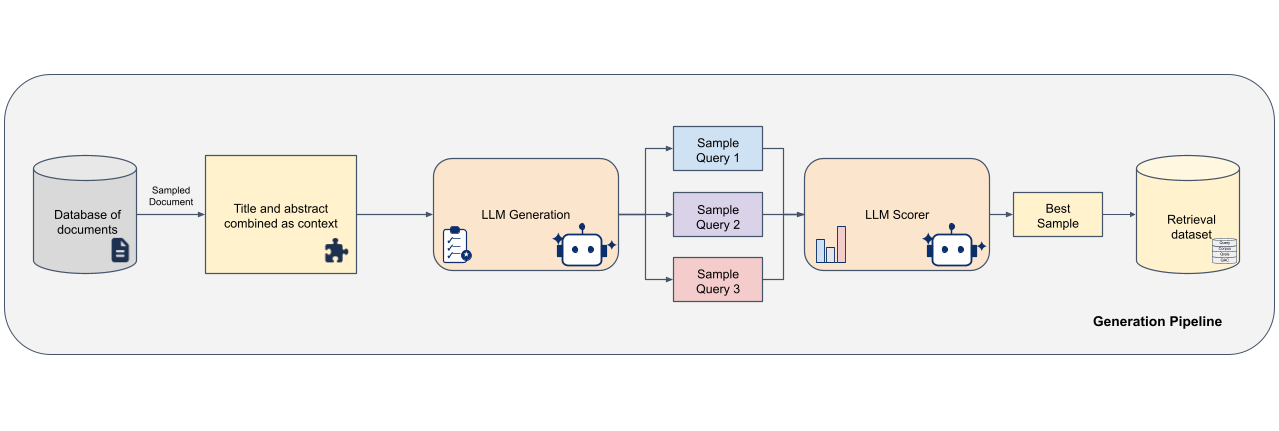
\includegraphics[width=0.98\textwidth]{multilingual_chemistry_retrieval_pipeline_EDITABLE.png}
    \caption{Overview of the QAC generation pipeline: source documents are
    converted into grounded candidate questions, scored, and exported as
    retrieval-ready records. Icons adapted from Font Awesome, licensed under CC BY 4.0. }
    \label{fig:qac-generation-flow}
\end{figure*}
\paragraph{Corpus and context construction.}
We build on two patent-derived corpora that contribute complementary kinds of
multilinguality. \textit{Google Patents} supplies scale and language breadth:
23{,}787 published applications, predominantly WIPO (WO, 15{,}048) and European
(EP, 4{,}610) filings, with a sizeable Mexican (MX, 3{,}952) share, spanning five
languages (English, French, Spanish, German, Chinese), from which we take the
title and abstract as the evidence block. On this side the non-English versions
are Google's \emph{machine} translations, and because Chinese coverage was zero
we machine-translated 400 documents to seed it using GPT 5.5. \textit{EPO} supplies clean
cross-lingual parallelism: 11{,}315 granted B1 specifications, each published as a
\emph{human}-translated English/German/French triple ($\approx$3{,}770 per
language) with professionally translated first claims, which we add to the
evidence block; we introduce no translations of our own on this side.


\paragraph{Candidate generation.}
For each source document we prompt \texttt{gpt-5-mini} to generate three
candidate questions, each grounded in a completely by the passage. (Table~\ref{tab:benchmark-stats} reports the
resulting counts). Two choices shape the query distribution. First, a question's
\emph{target language} is sampled per document relative to the languages that
document exists in: \emph{random-existing} picks a language the patent already
has a version in, so the query has a same-language answer;
\emph{random-missing} picks one it does \emph{not}, yielding a pure cross-lingual
``no-home'' query; and \emph{all} generates the question in every 5 languages
we targeted. Second, each question is written in one of two \emph{modes}:
\emph{technical} questions ask for a single concrete fact, a parameter,
material, outcome, method, or structural detail, answerable by the document, while \emph{general} questions ask about the document's problem, approach,
or application in deliberately paraphrased, low-overlap wording. The mode prompts
are written in the target language so questions read natively. The prompts (English version) are available in  Figures~\ref{fig:prompt-technical}
and~\ref{fig:prompt-general}.

\paragraph{Scoring, human audit.}
The three candidates per document are scored not by the generator but by a
separate verifier, \texttt{claude-sonnet-4.6}, which rates each candidate
on faithfulness and on mode-specific quality; we keep the highest-scoring
candidate per document.(verifier prompts in
Figures~\ref{fig:verifier-faith}--\ref{fig:verifier-general}). Because the
verifier is itself a model, we audited it against a 97-item human-annotated
sample using criteria that mirror the LLM rubric; three rounds of annotator
feedback further refined both the generation and the verifier prompts. On the
final sample the human mean is \textbf{8.33/10} (technical \textbf{8.72}, general
\textbf{7.91}) and \emph{no} item was rejected (none scored in the 0--3 band;
Figure~\ref{fig:human-scores}). We then export the standard retrieval
artifacts.


\section{Evaluation Setup}

TODO: Write this section from the paper plan.

\section{Results}

\subsection{Model Rankings and the Cross-Lingual Gap}


\begin{table*}[t]
\centering
\small
\setlength{\tabcolsep}{5pt}
\begin{tabular}{l ccc ccc ccc}
\toprule
 & \multicolumn{3}{c}{\textbf{Google Patents}} & \multicolumn{3}{c}{\textbf{EPO}} & \multicolumn{3}{c}{\textbf{Cross-lingual coverage}} \\
\cmidrule(lr){2-4}\cmidrule(lr){5-7}\cmidrule(lr){8-10}
Model & R@10 & CLIR & LT\% & R@10 & CLIR & LT\% & $k^\star_{80}$ & $k_{\mathrm{same}}$ & $k_{\mathrm{cross}}$ \\
\midrule
embeddinggemma            & \textbf{0.57} & \textbf{0.54} & 73          & \textbf{0.58} & \textbf{0.52} & 74          & \textbf{147}   & \textbf{36} & \textbf{121} \\
bge-m3                    & 0.51          & 0.47          & \textbf{74} & 0.55          & 0.47          & 66          & 304            & 66          & 215 \\
qwen3-0.6B                & 0.49          & 0.45          & 72          & 0.47          & 0.39          & 61          & 425            & 63          & 310 \\
nomic-v2-moe              & 0.46          & 0.41          & 63          & 0.51          & 0.43          & 63          & 367            & 55          & 321 \\
granite-278m              & 0.41          & 0.39          & 72          & 0.39          & 0.36          & 84          & $>$1000        & 641         & 569 \\
LaBSE                     & 0.30          & 0.27          & 59          & 0.27          & 0.25          & \textbf{85} & $>$1000        & 761         & $>$1000 \\
e5-large-instruct$^\dagger$ & 0.21        & 0.09          & 12          & 0.29          & 0.12          & 19          & $>$1000        & 47          & $>$1000 \\
SapBERT                   & 0.24          & 0.20          & 49          & 0.22          & 0.17          & 54          & $>$1000        & 807         & $>$1000 \\
\bottomrule
\end{tabular}
\caption{Retrieval performance on both patent offices. Best per column in bold.}
\label{tab:main-results}
\end{table*}

embeddinggemma leads on both offices and on every axis (Google Patents / EPO
Recall@10 0.57 / 0.58, CLIR@10 0.54 / 0.52) and reaches both golds the fastest
($k^\star_{80}{=}147$ vs.\ 304 for the next model), with bge-m3 a consistent second;
the ordering barely changes between the two offices, so it reflects the task ratherqwen3-0.6B and
nomic-v2-moe are mid-pack, while granite-278m, LaBSE and SapBERT trail by 20--30
Recall@10 points---and one model is an instructive outlier: e5-large-instruct looks
mid-pack on raw Recall@10 (0.21 / 0.29) but its CLIR@10 collapses to 0.09 / 0.12 and
its LT to 12 / 19, failing on cross lingual task. Off-the-shelf multilingual embedders are
therefore far from interchangeable on this task, and even the best absolute numbers
are low for an industrial deployment.


Across the whole field, retrieving a same-language copy of the answer is far easier
than retrieving its foreign twin and no model escapes the drop. The cross-lingual
coverage depths make the gap concrete: for the models that retrieve effectively the
same-language gold surfaces within a few dozen documents ($k_{\mathrm{same}}$
36--66) while its cross-language twin takes several hundred ($k_{\mathrm{cross}}$
121--321); for the weaker models both depths balloon and the cross-language gold is
frequently never covered for $80\%$ of queries within the retrieved top-1000. The
same pattern holds language by language: pooled across models, same-language recall
stays near 0.56--0.62 in every query language while cross-language recall sits around
0.34--0.38, a roughly 0.25 gap present in all five languages
(Figure~\ref{fig:home-advantage}); and the query$\times$document grid shows the loss lives off the diagonal for every
model (Figure~\ref{fig:qd-grid}): even the strongest retrievers fall to a fraction
of their same-language cell on individual routes, embeddinggemma drops from 0.69
same-language (English) to 0.18 when an English query must reach a German document,
bge-m3 from 0.62 (German) to 0.33 reaching a Spanish document, and nomic-v2-moe from
0.69 (French) to 0.12 reaching a Chinese one. Cross-linguality, not raw retrieval
power, is what every model struggles with.

\subsection{Alias-Graph: Inconsistency and Confusion}
\label{ssec:alias}

Asking the same compound in all five languages does not return the same patents.
The best cross-lingual RBO any model reaches is only 0.39 (embeddinggemma), a
ceiling no model beats (Figure~\ref{fig:alias}a), and it drops below 0.15 for the
weakest retrievers: two language variants of the same query share only a minority
of their top-ranked documents, so the embedding space is far from language-agnostic.


The second failure is chemical confusion: a wrong but chemically similar compound
out-ranks every gold patent on 14--48\% of queries depending on the model
(Figure~\ref{fig:alias}b, ALL column). The rate is strongly language-dependent, in
the direction the cross-lingual setting predicts. Averaged over models it is lowest
for English queries ($\approx$21\%) and highest for Chinese ($\approx$39\%), with
German, French, and Spanish in between ($\approx$28--30\%); the same chemical
question is markedly more likely to surface a look-alike above the right document
when it is asked in a lower-resource language than in English. The two failures
compound: a model that is both inconsistent across languages and easily confused by
near-neighbours is exactly the one a chemistry team must not deploy.

\begin{figure*}[t]
  \centering
  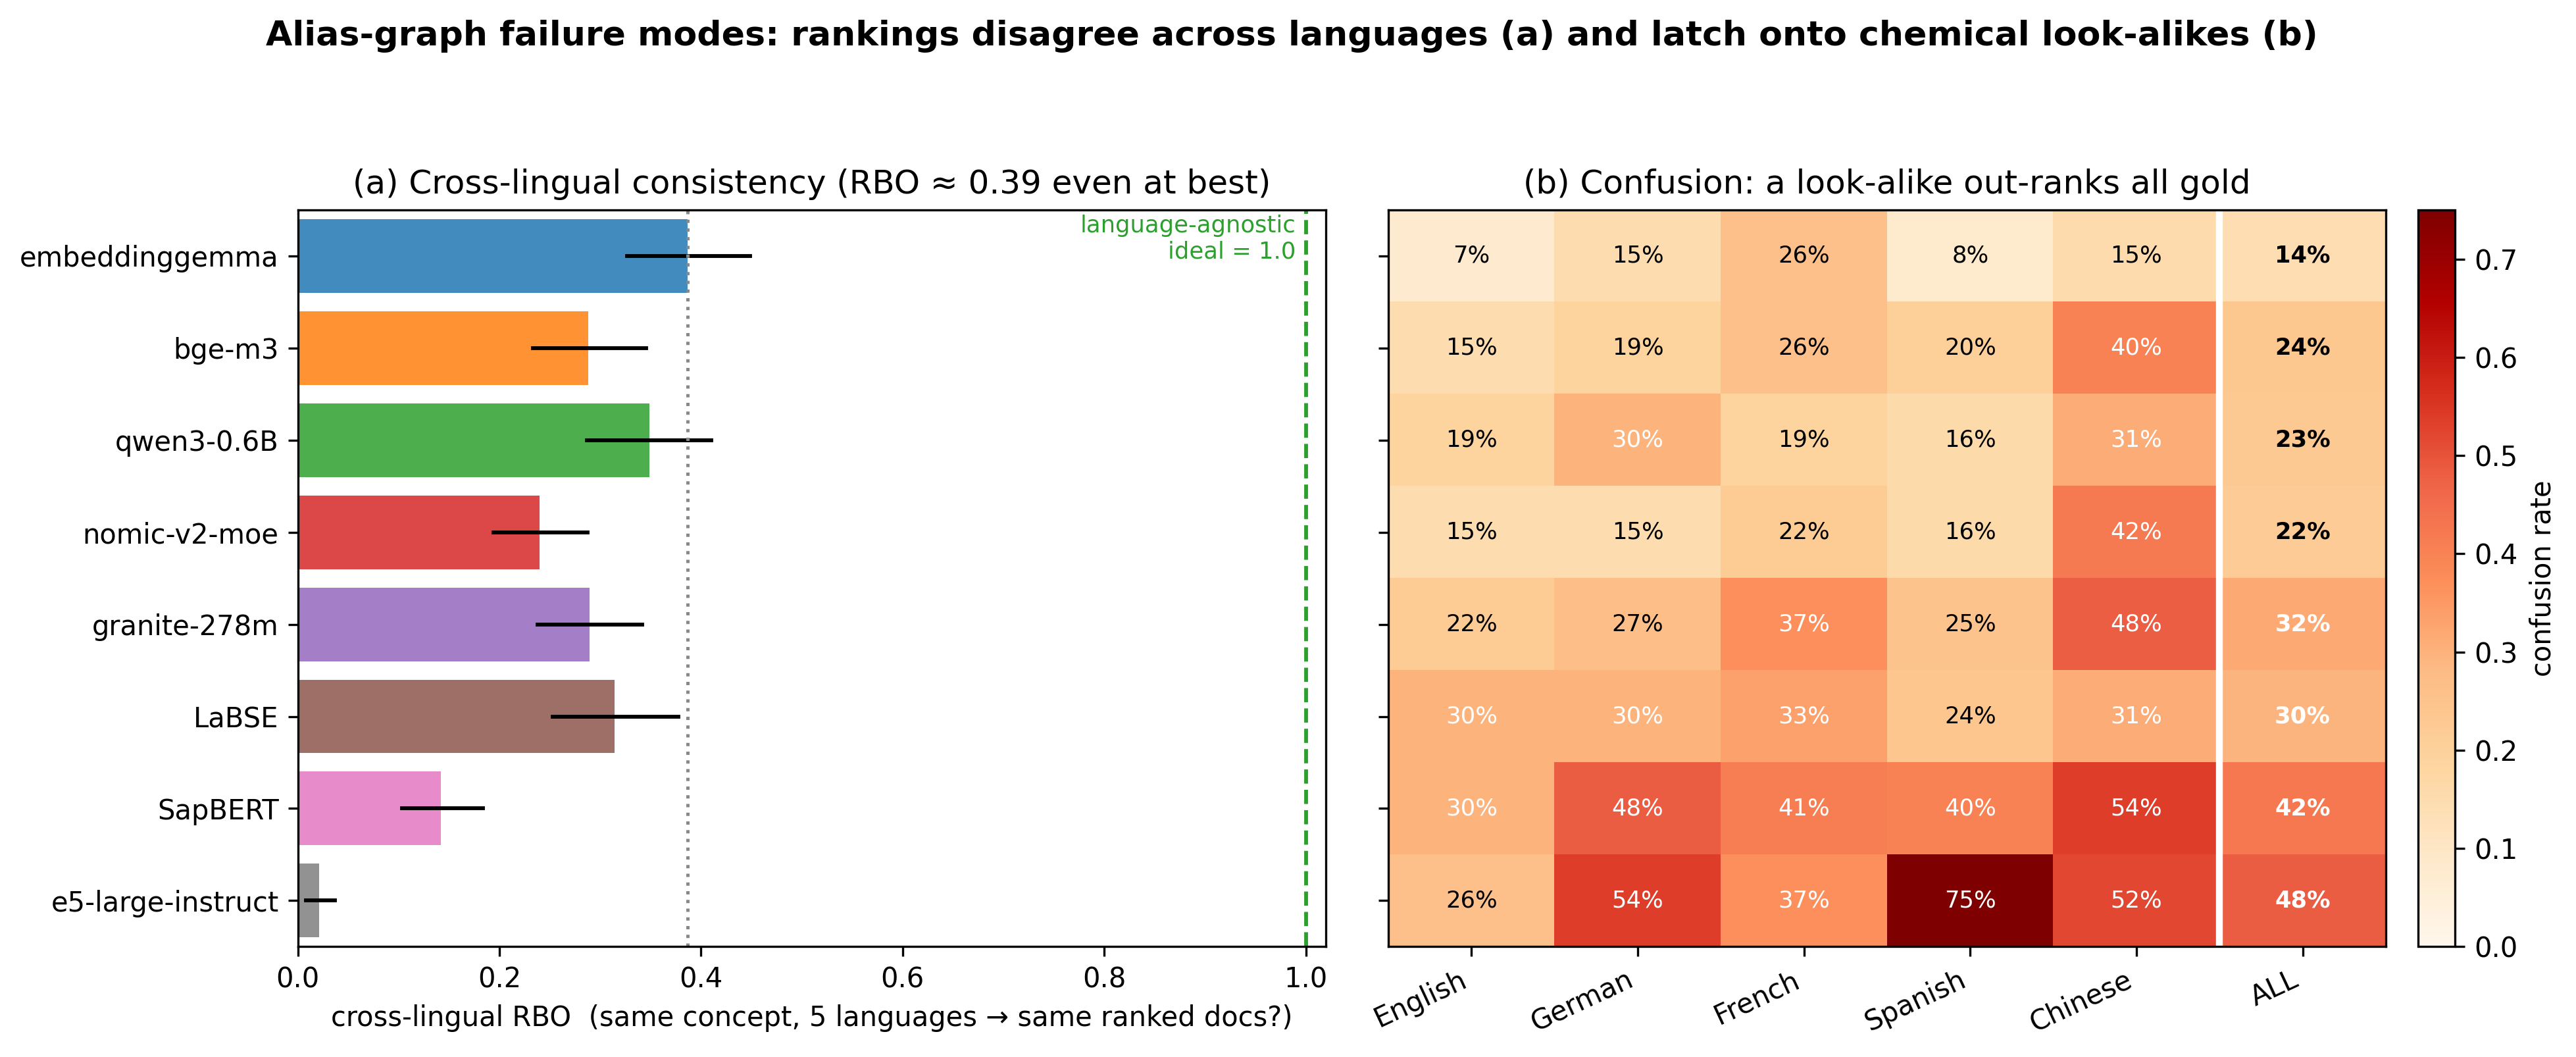
\includegraphics[width=\linewidth]{claimD_D6_rbo_publication.png}
  \caption{Alias-graph failure modes across the eight models. \textbf{(a)}~Cross-lingual
  RBO: how much the top-ranked lists for the same compound asked in five languages
  overlap ($1=$ identical, $0=$ disjoint); the most consistent model reaches only
  $0.39$. \textbf{(b)}~Confusion rate: how often a chemically confusable look-alike
  out-ranks every gold patent, by query language and pooled (ALL column);
  $14$--$48\%$ overall, lowest for English and highest for Chinese.}
  \label{fig:alias}
\end{figure*}



\subsection{Reading Cost and the Re-Ranking Ceiling}
XRC asks a concrete operational question: starting from the top of the ranked list,
how much further must a user read to reach the foreign-language version of the answer
than to reach a same-language copy? Panel~(a) of Figure~\ref{fig:cost} reports the
median, and it is never one: the cheapest model still reads about twice as deep
(LaBSE, 1.9$\times$) and the rest three to six times deeper (bge-m3 3.5$\times$,
embeddinggemma 5.0$\times$, nomic-v2-moe 6.0$\times$). A low reading cost is not a
virtue on its own, though, the cheapest readers here are the weakest retrievers,
which read shallow only because they surface so little, so XRC has to be read together
with capability (CLIR@10), not minimized in isolation. We drop e5-large-instruct from
all three panels because it fails the CLIR@10 $<0.10$ degeneracy gate: it almost never
retrieves a foreign twin at all, so its reading-depth ratio explodes (median
161$\times$) and its recoverability curve rests on mostly censored ranks, the
instruments are undefined for a model that does not retrieve the thing whose depth
they measure.


The other two panels ask what a downstream re-ranker could do about the buried
cross-language documents. A re-ranker only reorders the candidate pool it is handed,
so RRC@$K$ (panel~b) the fraction of cross-lingual queries whose first cross-language
gold (the answer's document in another language) has appeared by rank $K$, is a hard
ceiling on what re-ranking can recover: anything past depth $K$ is invisible to a
top-$K$ re-ranker. Two things stand out. First, the recoverable documents are
front-loaded: the knee $K^\star$, the point of sharpest diminishing returns on the
curve, sits at $2$--$5$ for the strong models, so a shallow top-5 pool already captures
the bulk of the cheaply recoverable cross-language gold (embeddinggemma RRC@5 $=0.53$);
a deeper pool keeps helping but with falling efficiency per decade (RRC@100 $=0.78$,
RRC@1000 $=0.93$), while the weak LaBSE and SapBERT reach their knee only at depth
$75$--$150$. Second, even an exhaustive re-ranker over the full retrieved pool hits a
wall: panel~(c) splits each model's cross-lingual shortfall into what a cheap top-10
re-rank recovers, what a deeper pool up to top-1000 adds, and an alignment-only floor
beyond the top-1000, cross-language gold that first-stage retrieval never surfaces and
that no re-ranker over the retrieved candidates can reach. That floor is $7\%$ of the
gap for embeddinggemma and grows to $27\%$ for SapBERT: the weaker the model, the more
of its cross-lingual failure is structural. And a realistic top-100 re-ranker recovers
even less, bounded by RRC@100 ($0.78$ for the best model), it reorders only what
first-stage retrieval already placed in its pool, so the durable fix for the residual
gap is representation alignment at indexing time, not a re-ranker at query time.



\begin{figure*}[t]
  \centering
  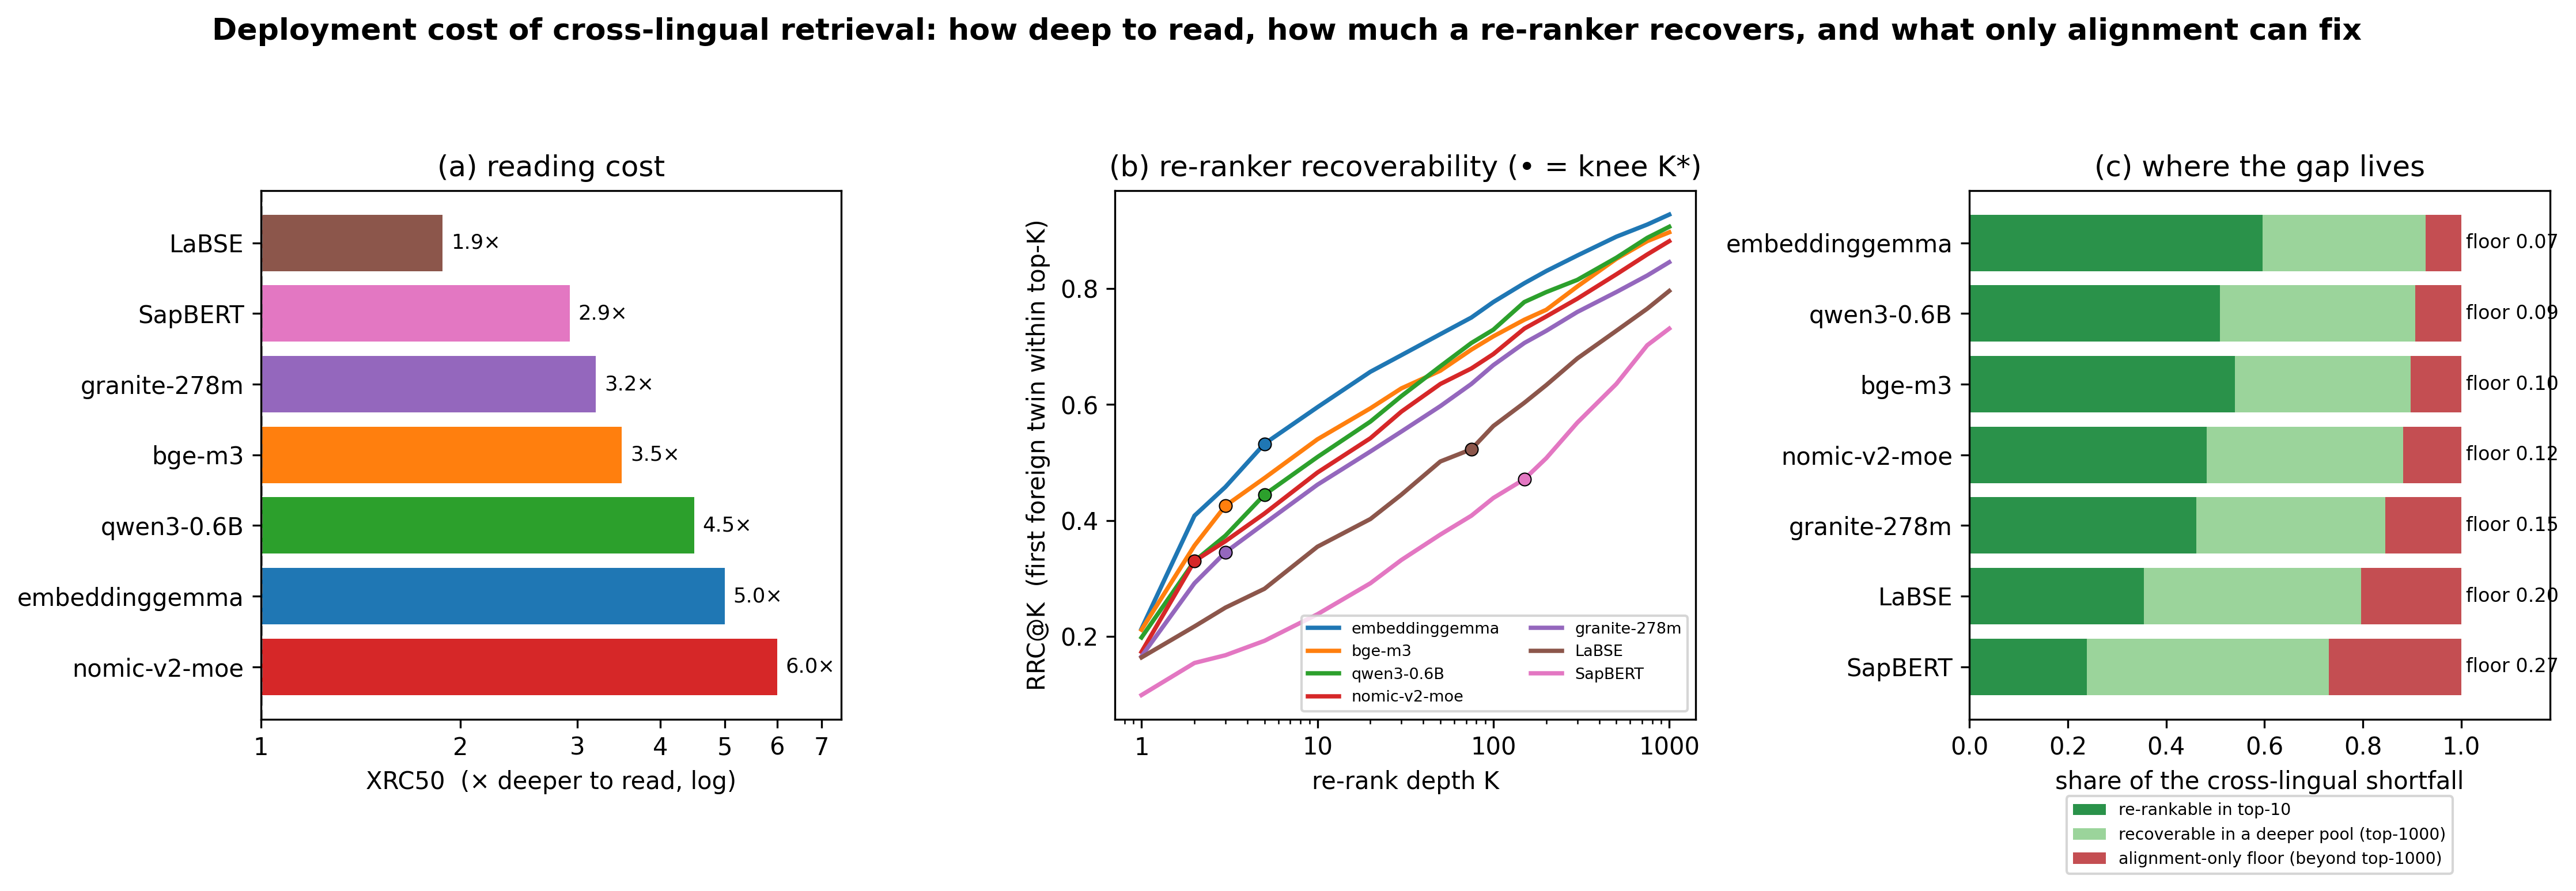
\includegraphics[width=\linewidth]{figures/claimE_E2_triptych.png}
  \caption{Deployment cost of cross-lingual retrieval (e5-large-instruct excluded by
  the CLIR@10 $<0.10$ gate). \textbf{(a)}~XRC50 reading cost; \textbf{(b)}~RRC@$K$
  re-ranker recoverability with knee $K^\star$ ($\bullet$); \textbf{(c)}~the shortfall
  split into re-rankable (top-10), deeper-pool (top-1000), and an alignment-only floor.}
  \label{fig:cost}
\end{figure*}

\section{Conclusion}

Multilingual chemistry retrieval needs evaluation data that makes the right
failure modes visible. In this paper, we presented a QAC generation and
validation pipeline for building such data, released it in retrieval-ready form,
and used it to evaluate dense multilingual retrievers beyond aggregate recall.
The central lesson is simple: a model that looks effective on average may still
prefer same-language shortcuts or chemically plausible but wrong documents over
the intended cross-language evidence.

The benchmark shows how to make those failures measurable. Language metadata
separates same-language from cross-language relevance; QAC provenance makes
generated queries auditable; human validation checks the LLM-based verifier; and
alias-graph hard negatives expose chemistry-specific confusions. These pieces
are useful beyond the particular patent-derived corpus used here: they provide a
template for building specialized multilingual retrieval evaluations in
high-trust technical domains.

For practitioners, the recommendation is to report robustness next to recall.
For benchmark builders, the recommendation is to start from the workflow failure
and preserve enough metadata to diagnose it. In multilingual chemistry search,
that means asking not only whether a relevant document was retrieved, but
whether the system found the intended evidence across language and chemical
confusability boundaries.

\section*{Limitations}

This benchmark is intentionally specialized. Chemistry patents provide a useful
substrate for controlled multilingual technical evidence, but results may not
transfer directly to other scientific domains, regulatory corpora, or general
web retrieval. Patent publication variants also give stronger content control
than unrelated multilingual corpora, but they do not guarantee full claim-level
equivalence across every language version. The design should therefore be read
as a reusable evaluation pattern, not as proof that the same model ordering will
hold everywhere or that all patent variants are legally interchangeable.

The QAC pipeline relies on LLM generation and LLM-based verification. Human
review supports the usefulness of the generated data, but the validation sample
is limited and does not replace expert patent or chemistry review for every
item. Future versions should expand expert annotation, especially for borderline
chemical relevance and hard-negative severity.

Finally, the current paper focuses on multilingual retrieval and alias-graph
confusability. Code-switching and noisy-query infrastructure exist in the
project, but we do not claim complete results for those settings here.


\clearpage
\bibliography{custom}

\clearpage 
\appendix % Supplementary figure and table numbering 
\setcounter{figure}{0} \setcounter{table}{0} \renewcommand{\thefigure}{S.\arabic{figure}} \renewcommand{\thetable}{S.\arabic{table}} % Unique internal identifiers for hyperlinks 
\renewcommand{\theHfigure}{supp.\arabic{figure}} \renewcommand{\theHtable}{supp.\arabic{table}}
\section{Appendix}

This appendix collects supporting analyses that are useful for interpretation
but too detailed for the six-page body.

\section{Additional Cross-Lingual Retrieval Diagnostics}

These diagnostics expand the paper's main cross-language retrieval result. They
show that the same-language advantage is not a single-score artifact: it appears
as model-level home advantage, directed language-pair asymmetry, delayed recovery
of multilingual publication variants, and weaker embedding separability for
cross-language gold evidence.

\begin{figure}[t]
  \centering
  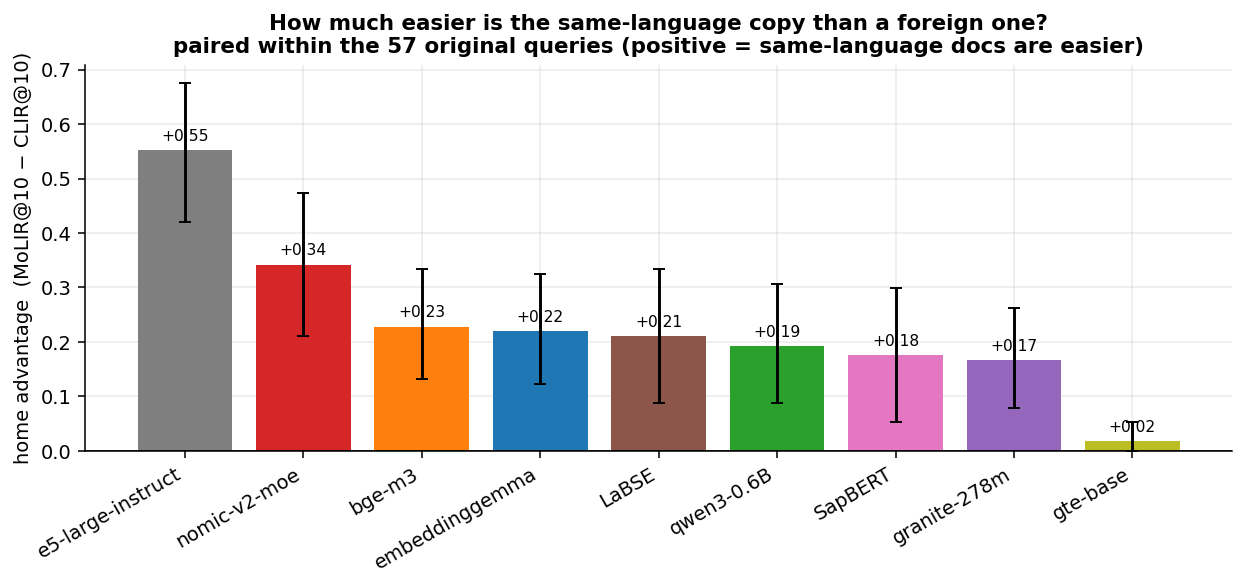
\includegraphics[width=\linewidth]{cp_fig02_home_advantage.png}
  \caption{Same-language home advantage by model. The gap between
  same-language and cross-language retrieval is the main reason aggregate recall
  can overstate deployment readiness.}
  \label{fig:app-home-advantage}
\end{figure}

\begin{figure}[t]
  \centering
  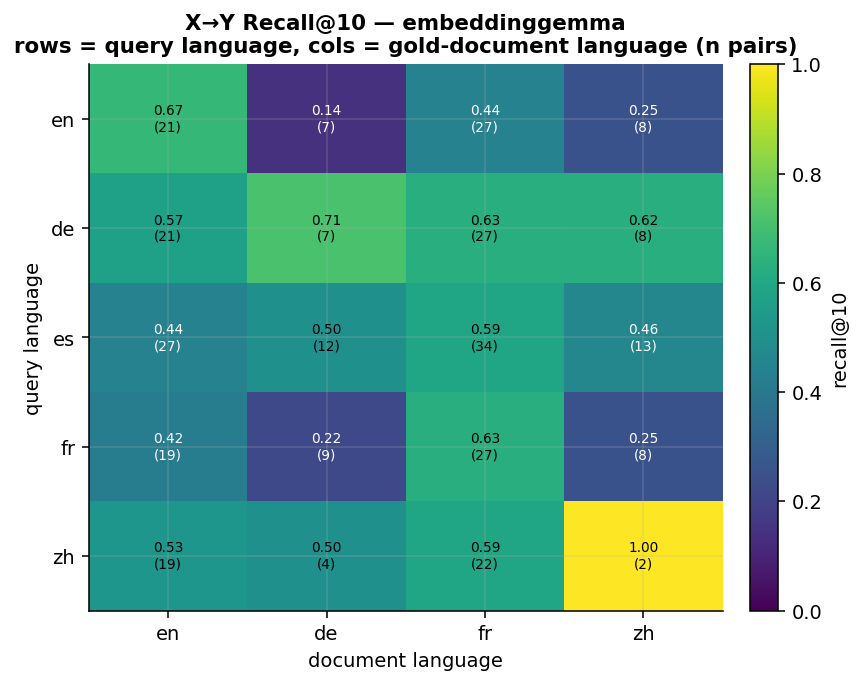
\includegraphics[width=\linewidth]{cp_fig03_directional_clir_matrix.png}
  \caption{Directional query-language $\rightarrow$ document-language retrieval.
  Cross-language retrieval is not symmetric: a model's behavior depends on both
  the query language and the target document language.}
  \label{fig:app-directional-clir}
\end{figure}

\begin{figure}[t]
  \centering
  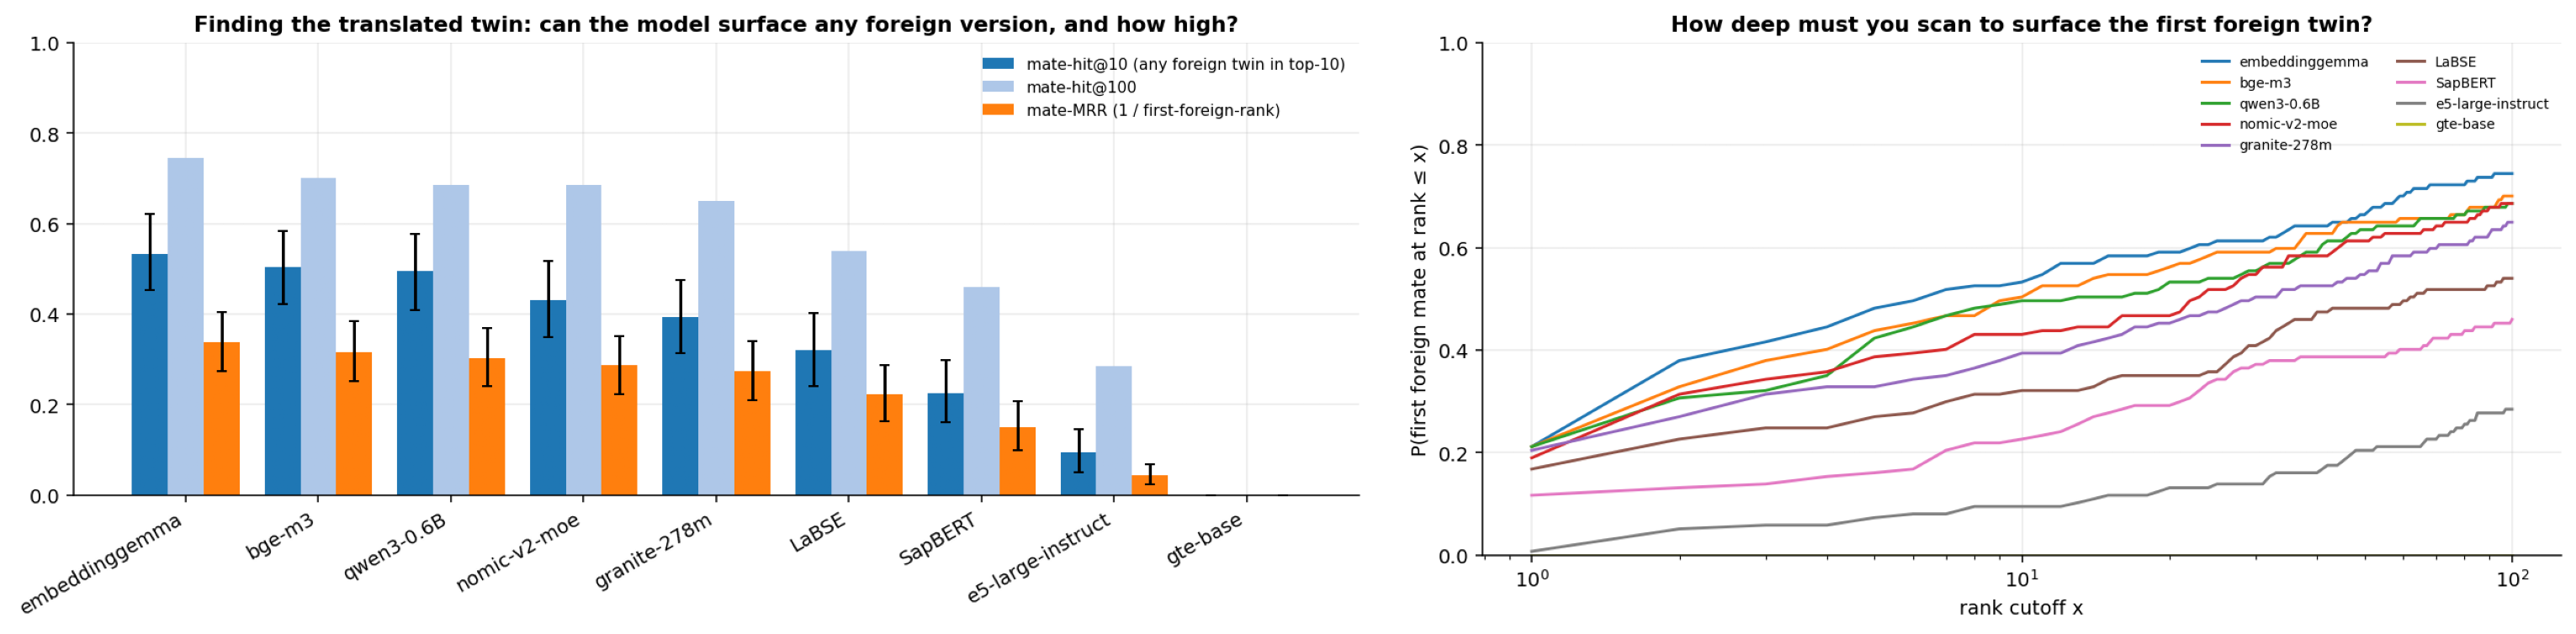
\includegraphics[width=\linewidth]{cp_fig06_07_mate.png}
  \caption{Foreign-twin retrieval diagnostics. The figure reports whether
  multilingual publication variants are found and how deeply a model must search
  before reaching the first cross-language twin.}
  \label{fig:app-mate-retrieval}
\end{figure}

\begin{figure}[t]
  \centering
  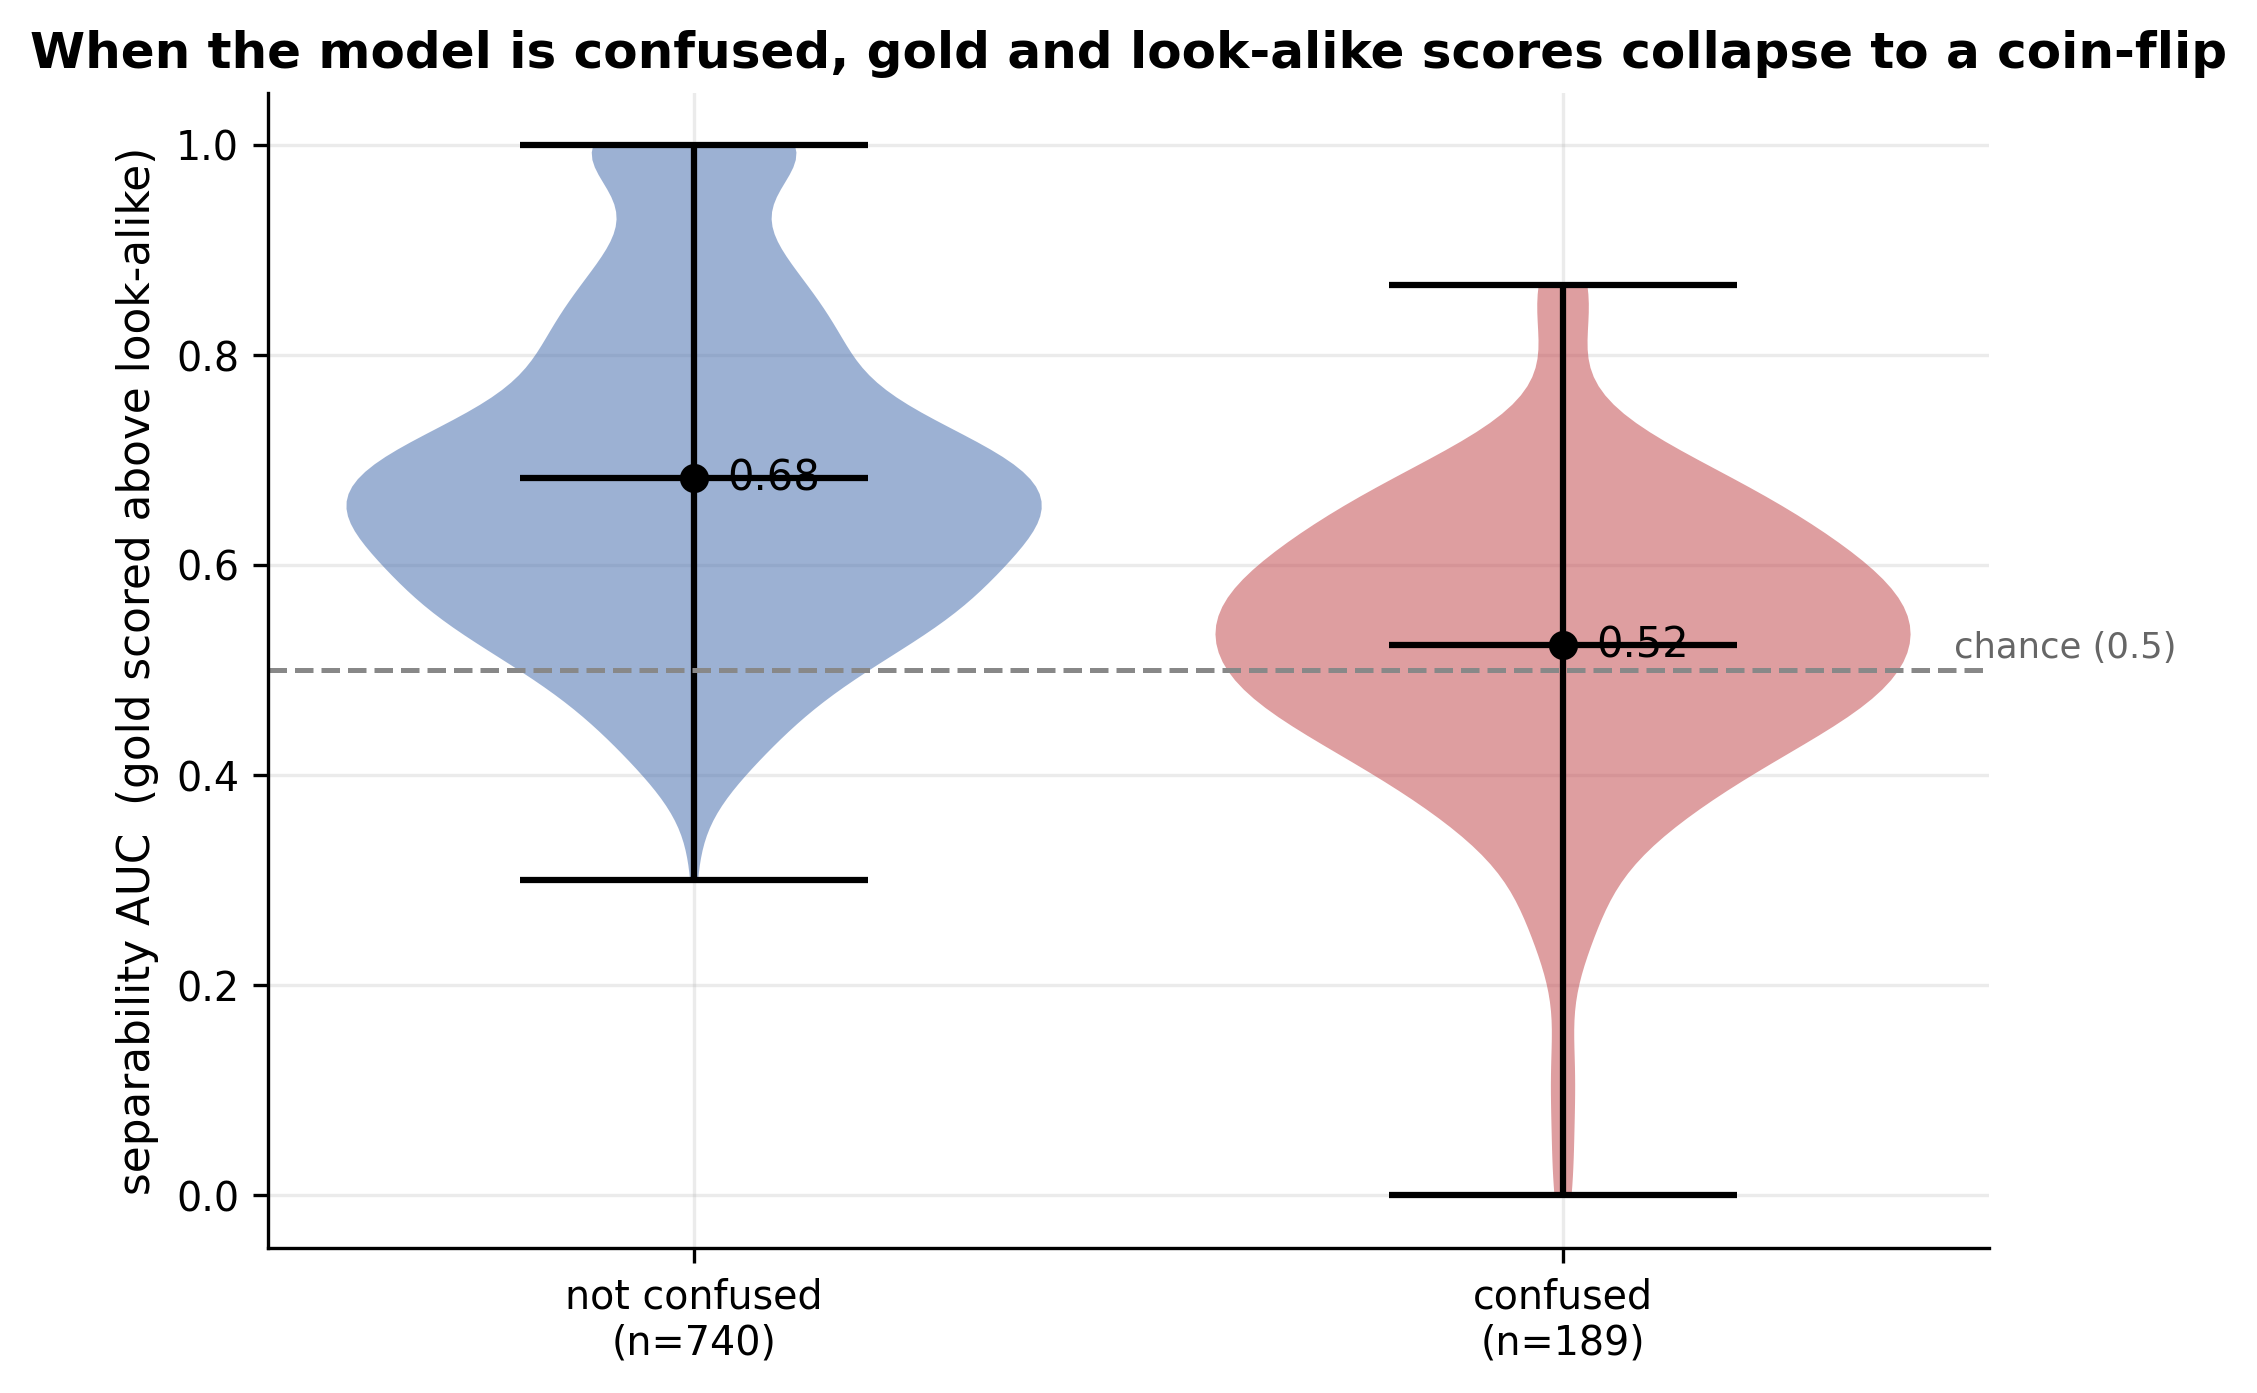
\includegraphics[width=\linewidth]{cp_fig11_separability.png}
  \caption{Embedding separability for same-language and cross-language gold
  documents. Lower cross-language separability indicates that the retrieval
  failure is partly representation-level, not only a top-$k$ ranking artifact.}
  \label{fig:app-separability}
\end{figure}

\section{Additional Alias-Graph Diagnostics}

The alias-graph analyses isolate the chemistry side of the retrieval problem.
They test whether multilingual queries for the same concept produce consistent
rankings and whether chemically plausible neighbors become systematic
distractors. Together, these figures explain why relevance in chemistry search
cannot be reduced to topical similarity alone.

\begin{figure}[t]
  \centering
  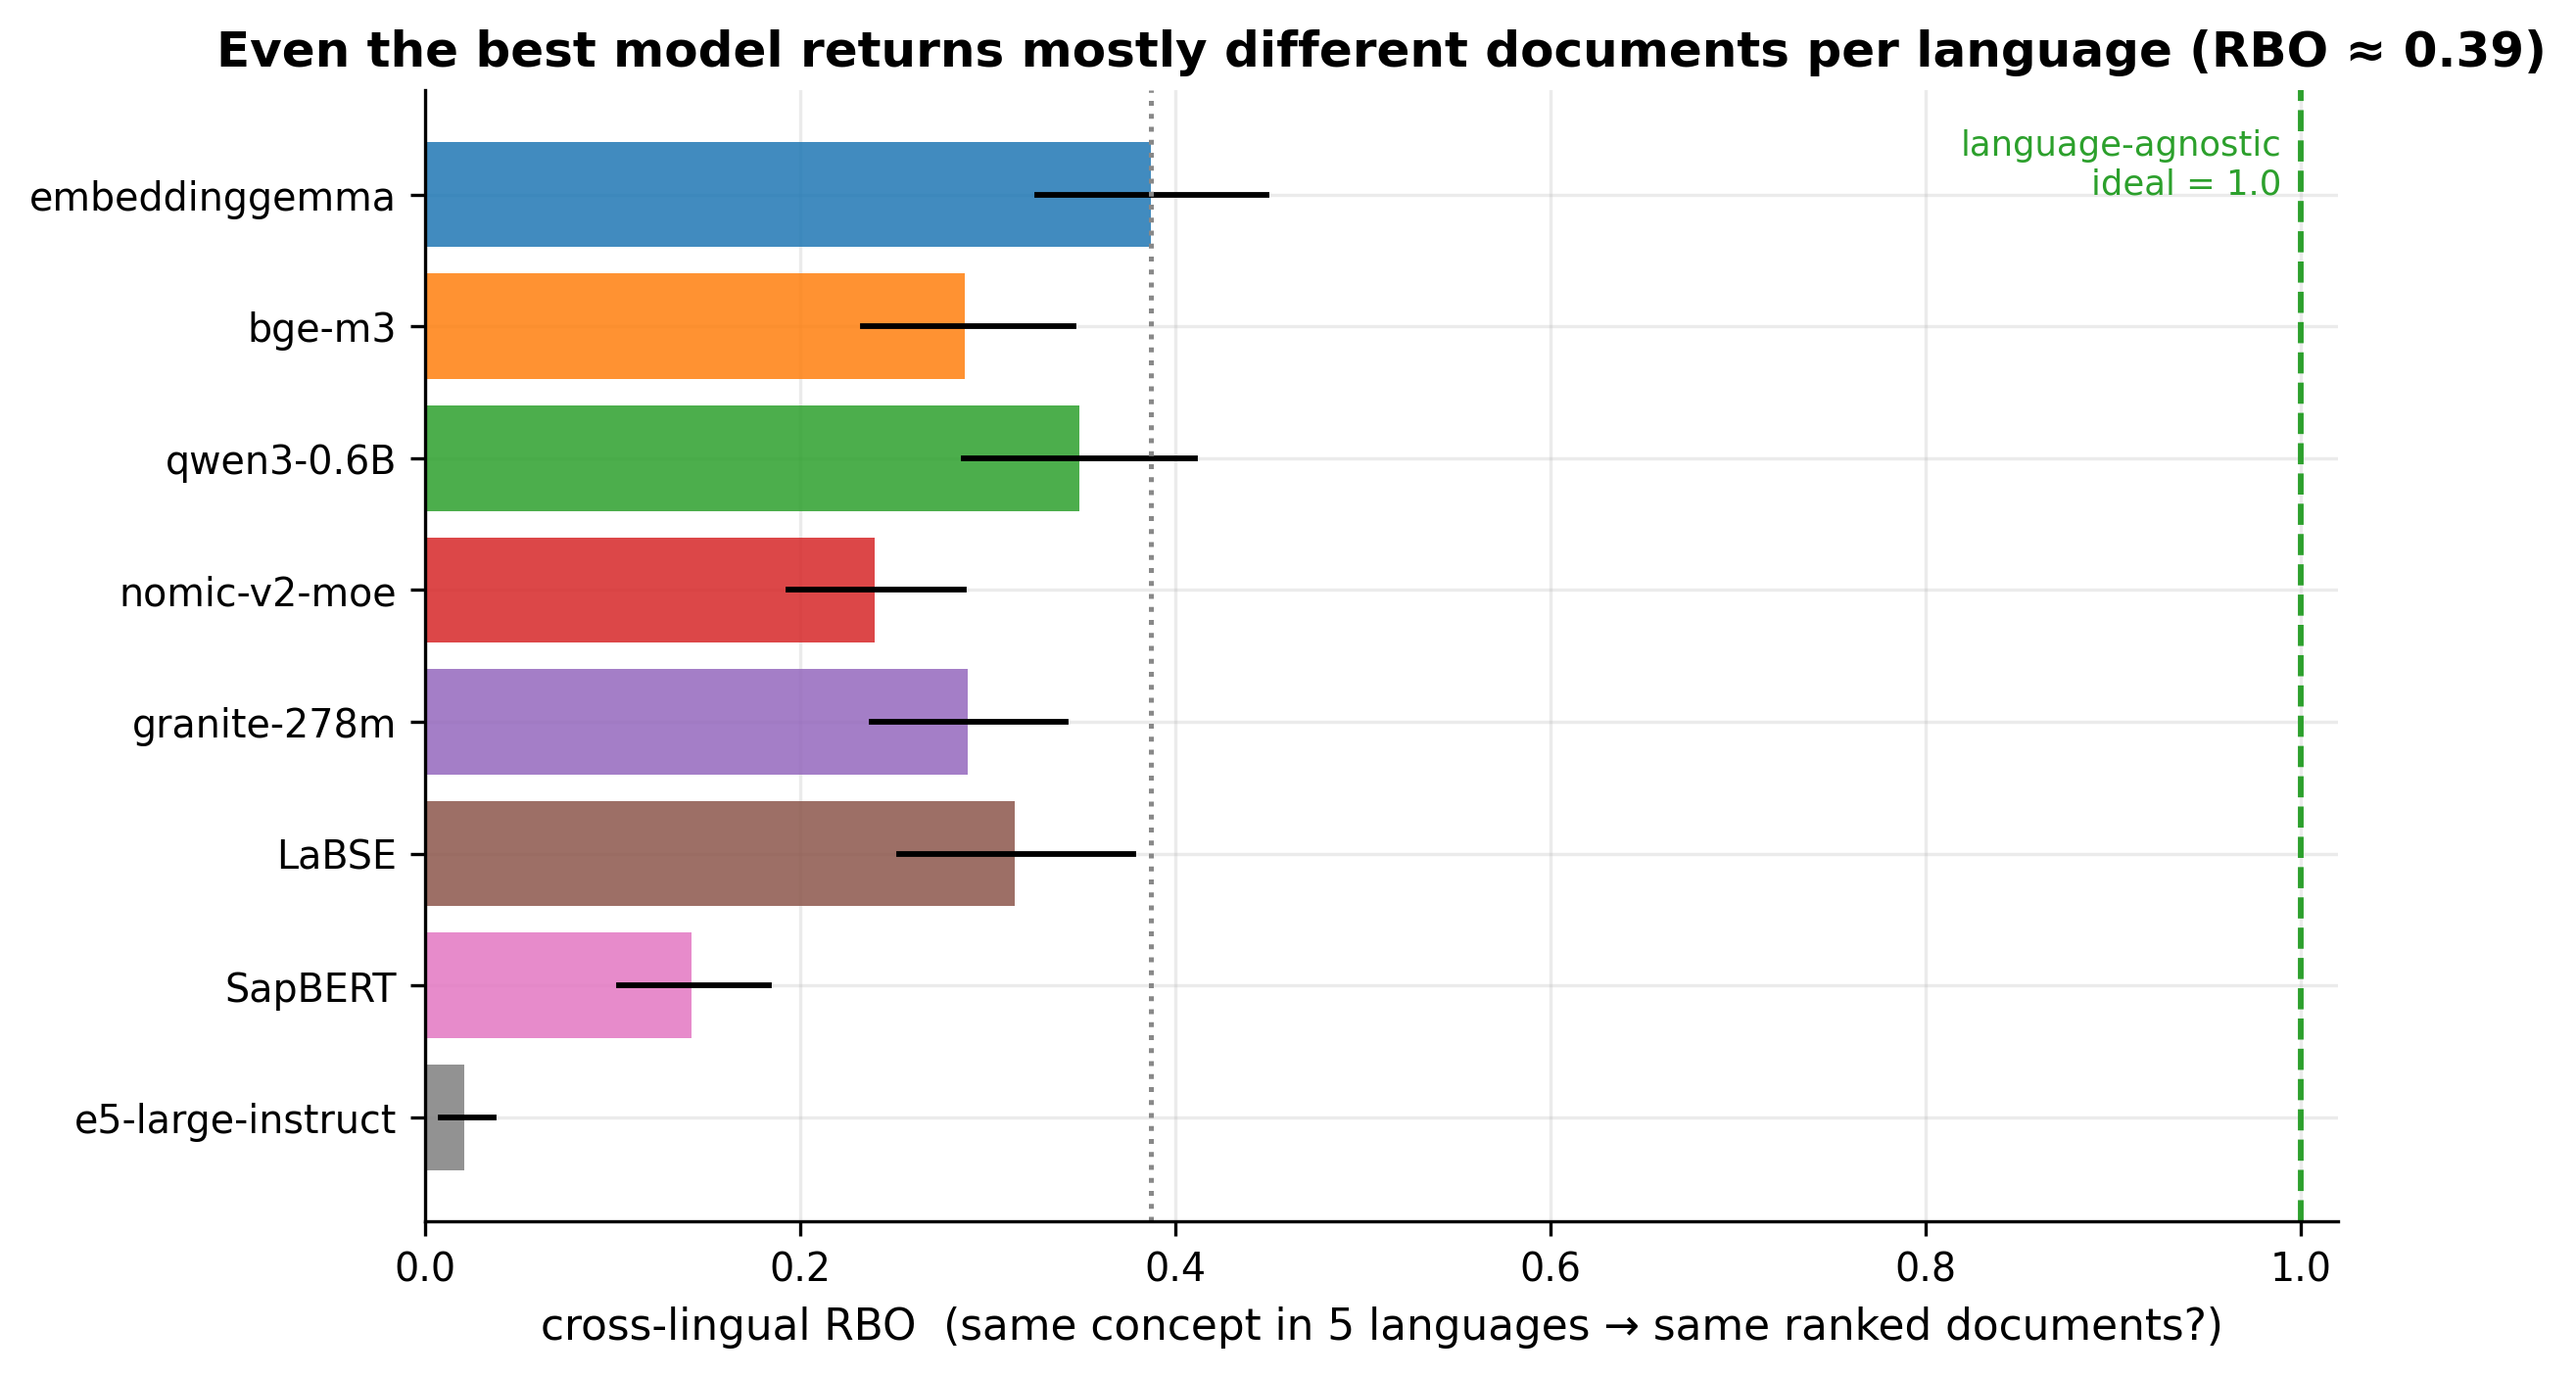
\includegraphics[width=\linewidth]{ag_fig1_cross_lingual_rbo.png}
  \caption{Cross-lingual ranking consistency for the same chemical concept asked
  in multiple languages. Low overlap means language variants of the same query
  can return substantially different ranked lists.}
  \label{fig:app-alias-rbo}
\end{figure}

\begin{figure}[t]
  \centering
  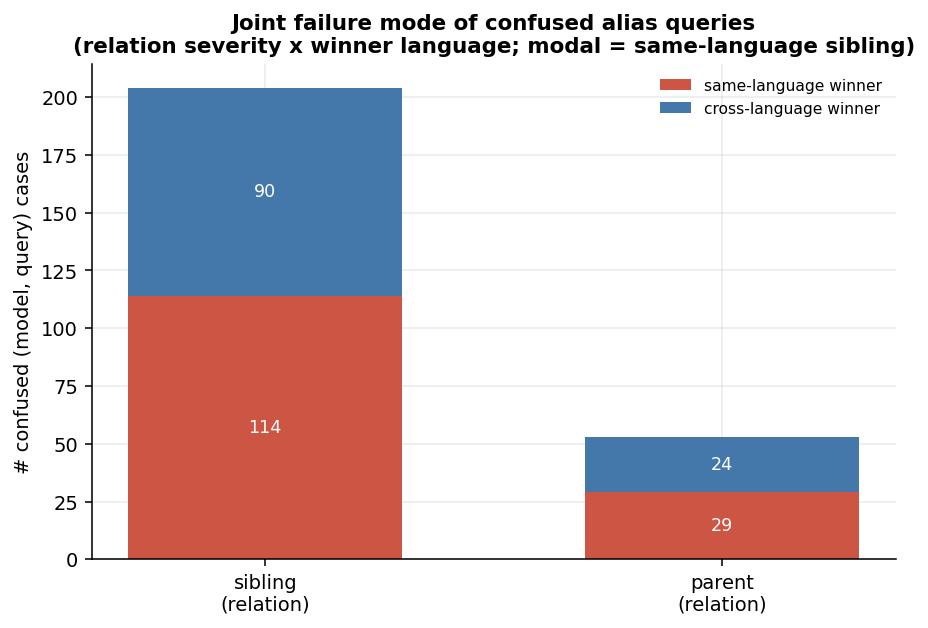
\includegraphics[width=\linewidth]{ag_fig12_joint_failure_modes.png}
  \caption{Joint language and chemistry failure modes among confused cases. This
  analysis links the paper's two central risks: same-language preference and
  chemically plausible but wrong neighbors.}
  \label{fig:app-joint-failures}
\end{figure}

\begin{figure}[t]
  \centering
  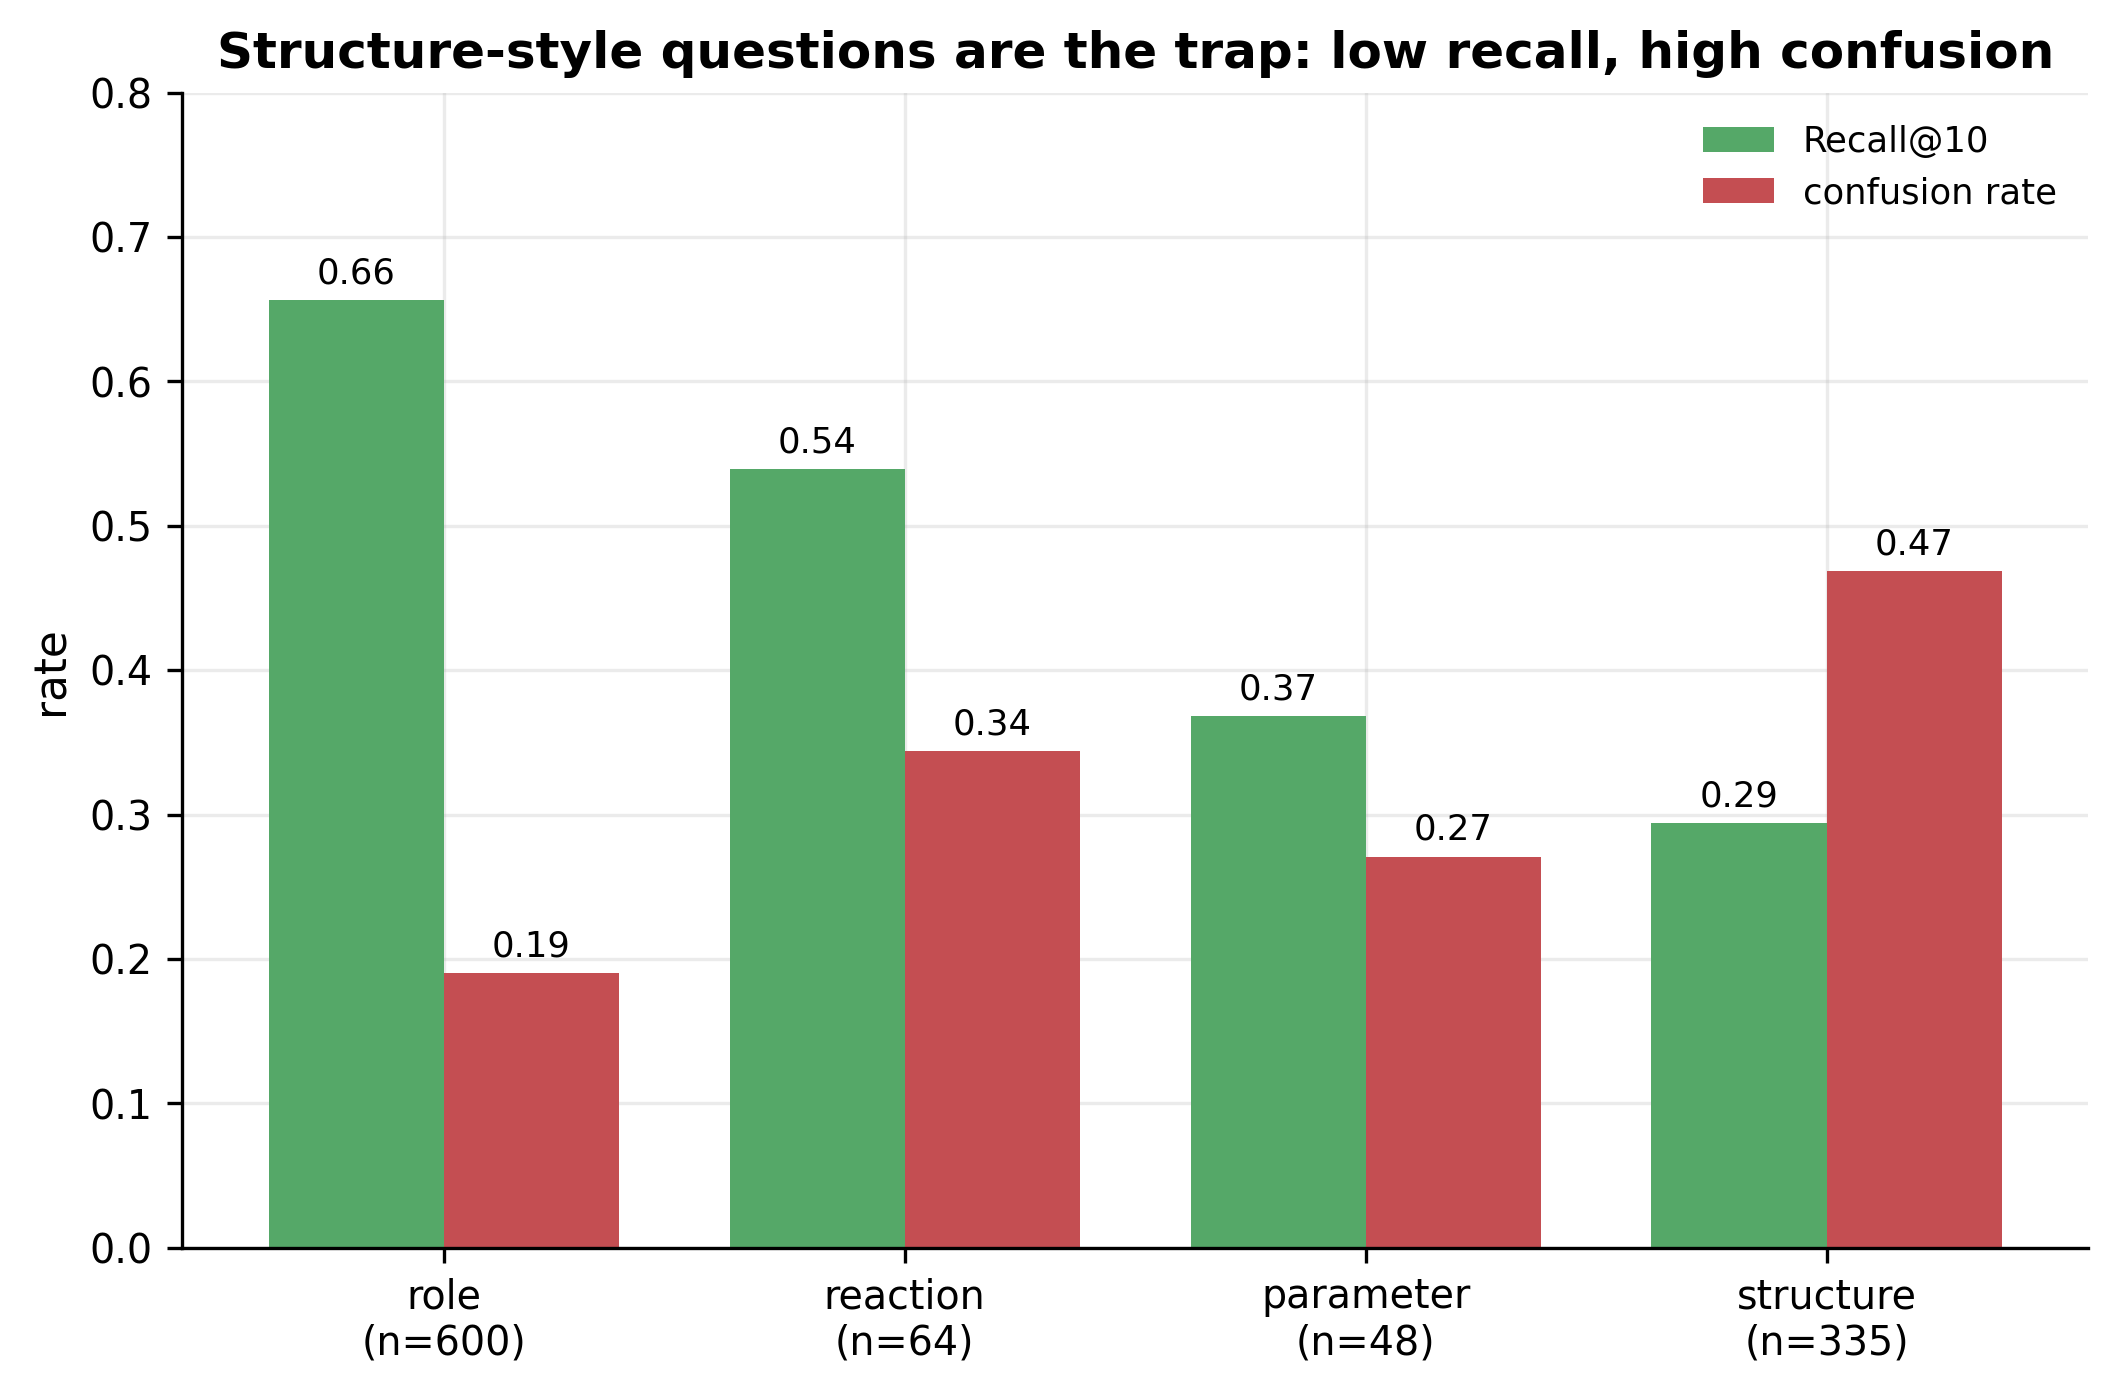
\includegraphics[width=\linewidth]{ag_fig6_question_type_effect.png}
  \caption{Question-type effects in the alias-graph benchmark. Some query types
  are substantially more vulnerable to chemistry-confusability than others.}
  \label{fig:app-question-type}
\end{figure}

\begin{figure}[t]
  \centering
  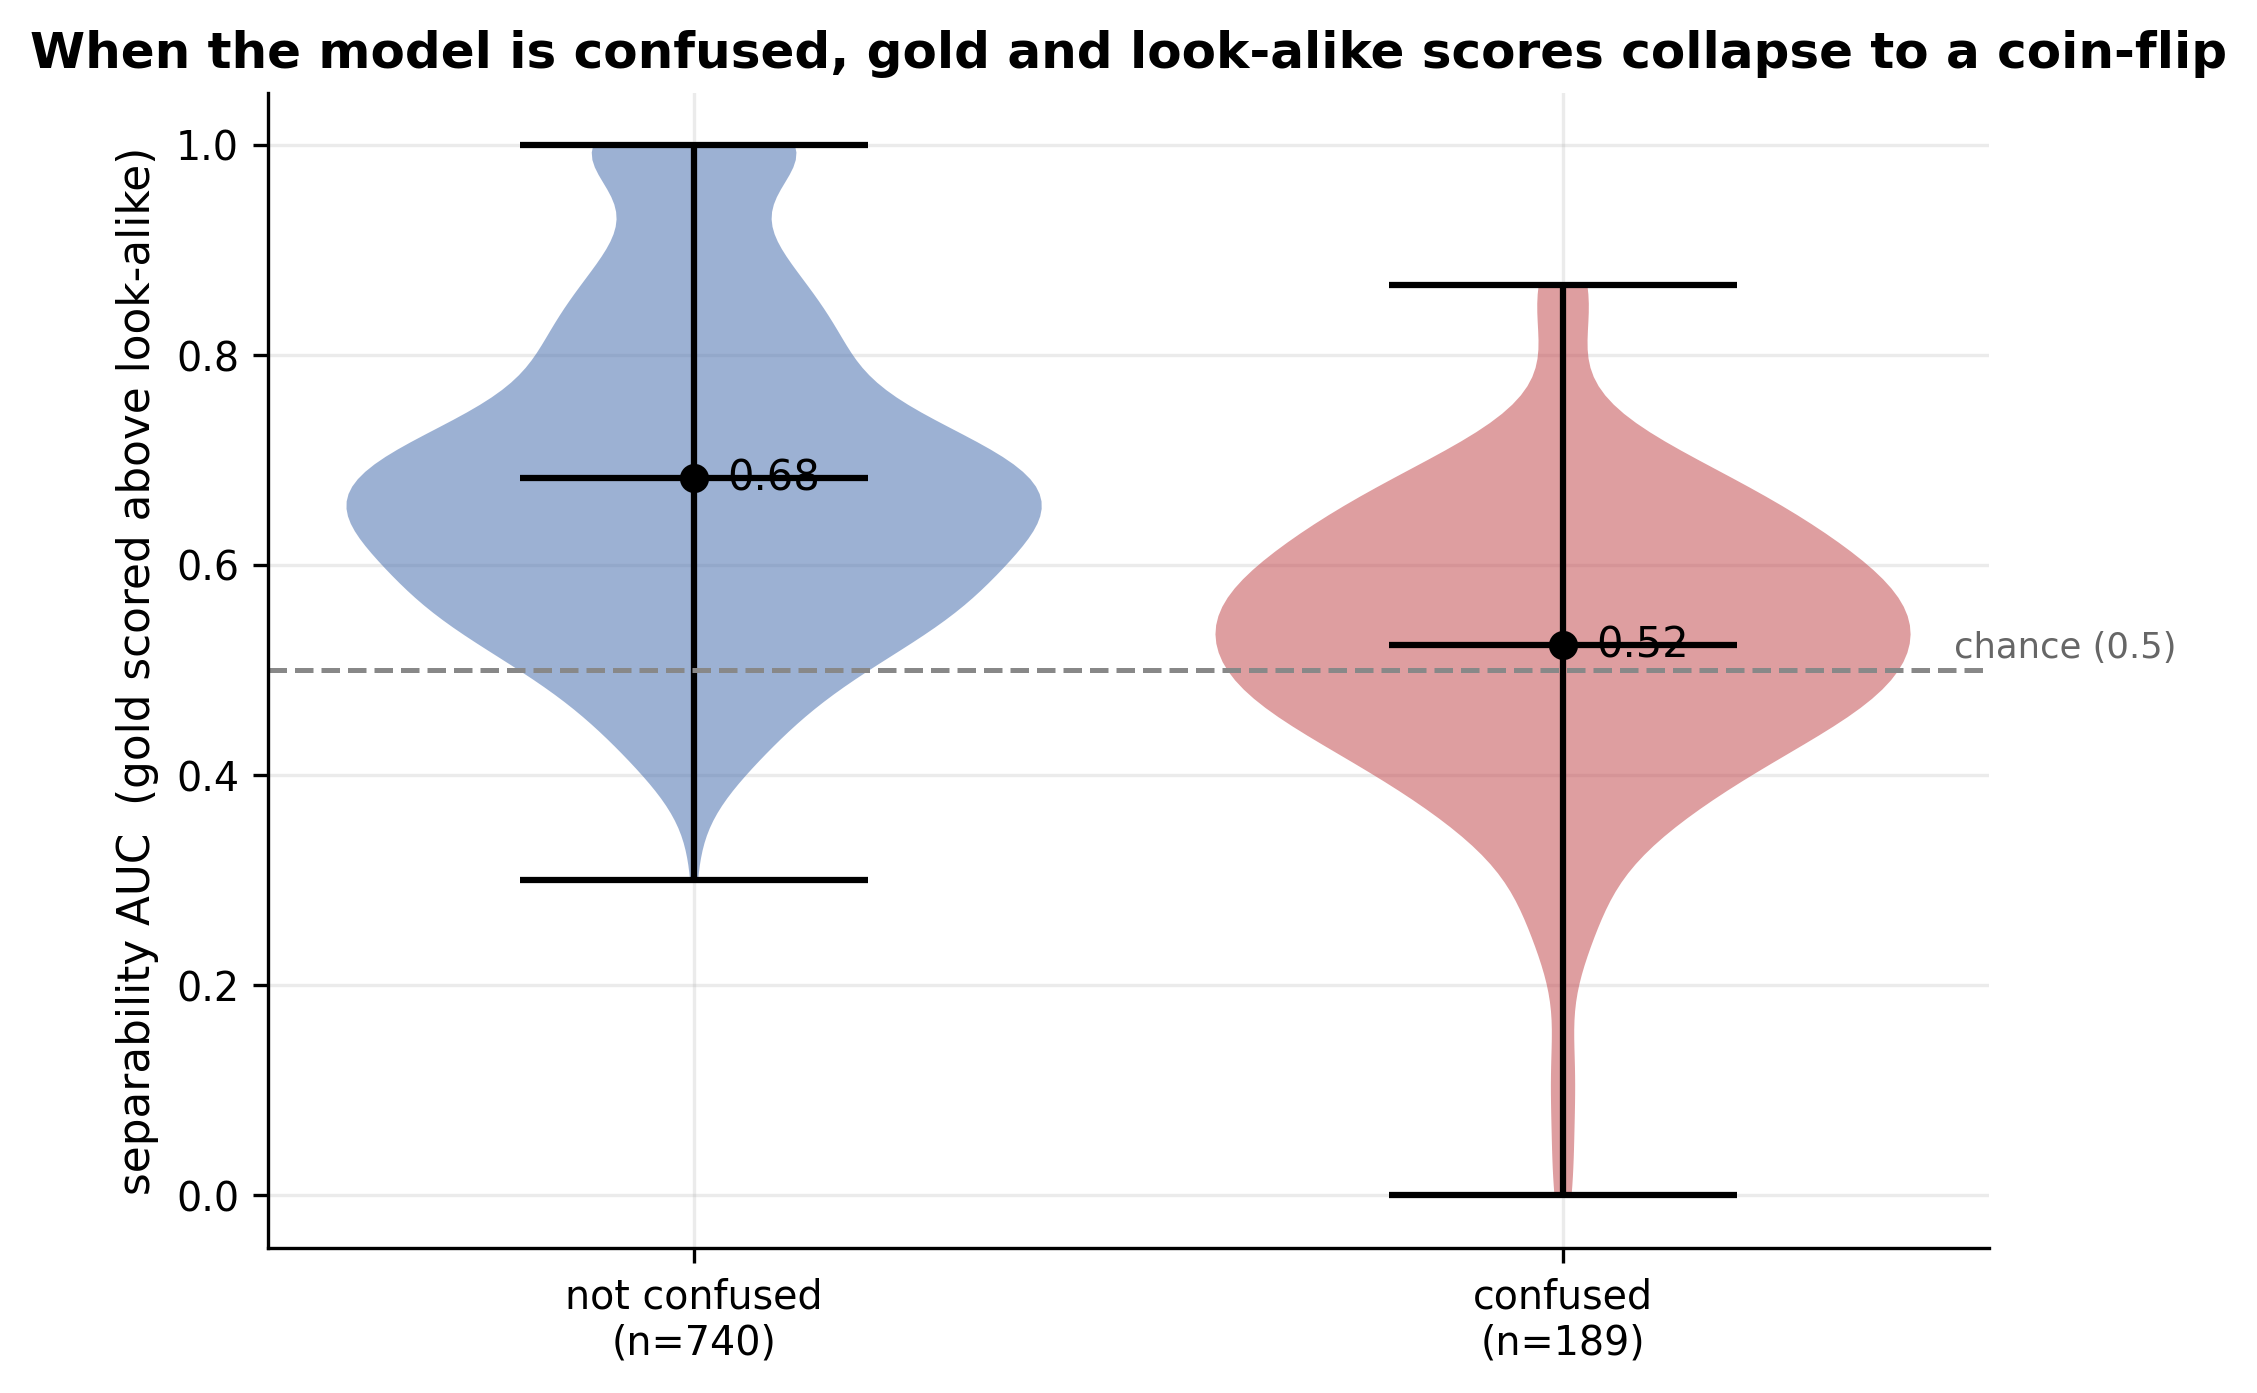
\includegraphics[width=\linewidth]{ag_fig8_confusion_is_separability.png}
  \caption{Confusion as separability collapse. Confused examples have weaker
  embedding separation between gold and non-gold documents.}
  \label{fig:app-confusion-separability}
\end{figure}

\begin{figure}[t]
  \centering
  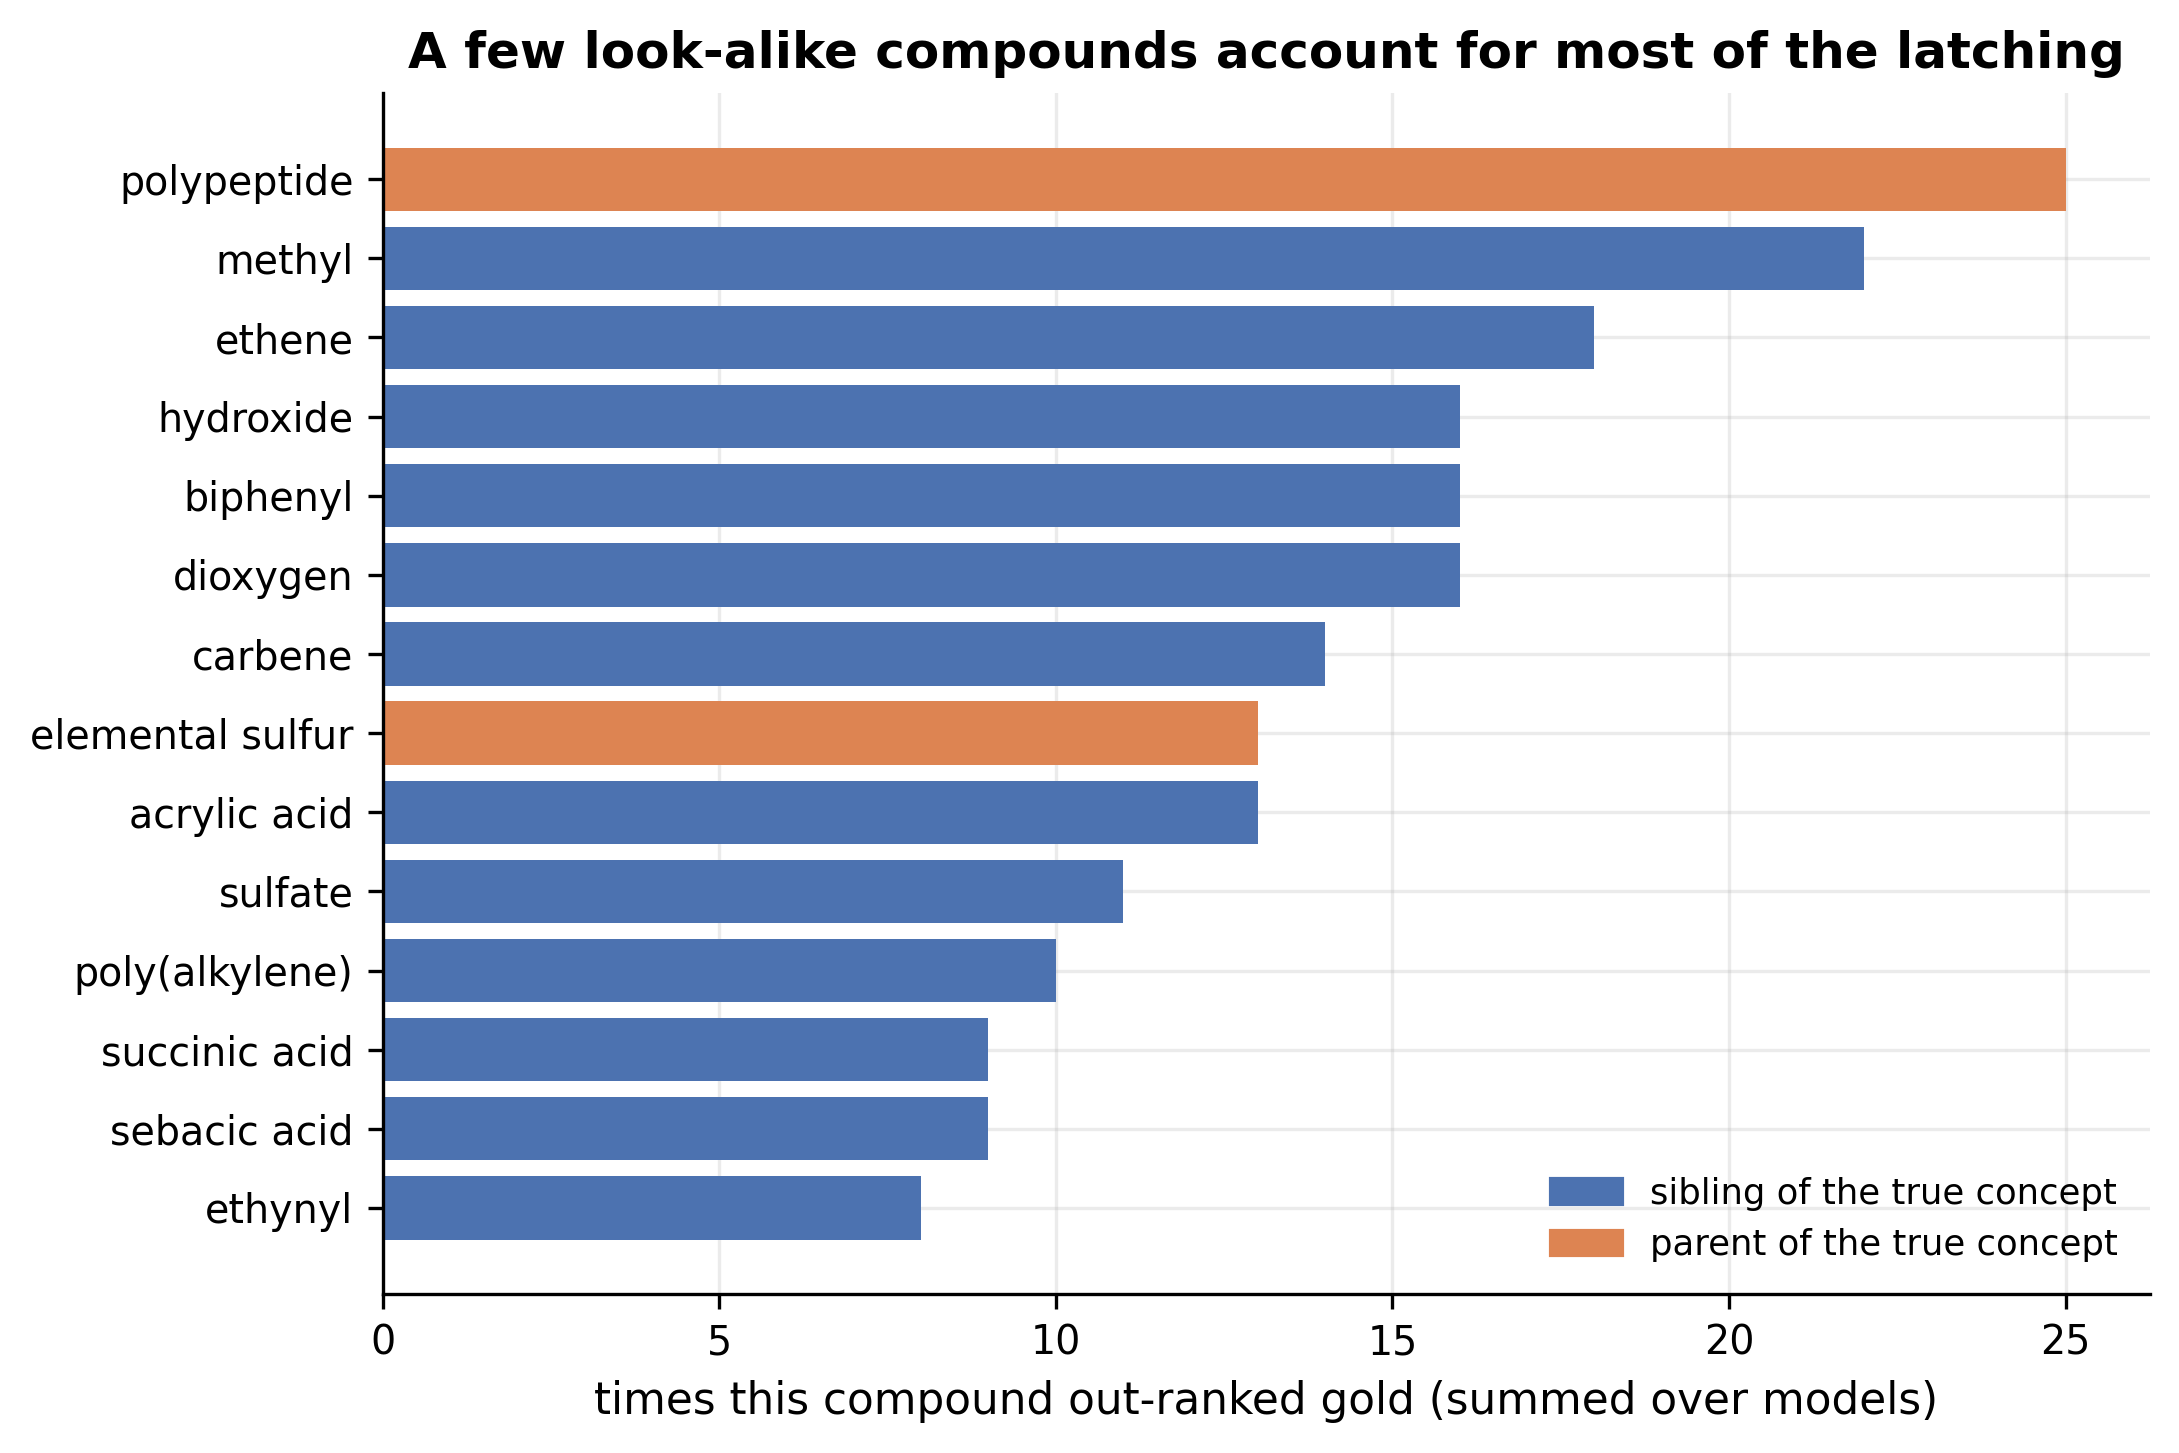
\includegraphics[width=\linewidth]{ag_fig5_universal_attractors.png}
  \caption{Universal attractors in the alias graph: chemically plausible
  look-alikes that repeatedly steal top rank across models or languages.}
  \label{fig:app-universal-attractors}
\end{figure}

\section{Deployment-Oriented Supporting Analyses}

These figures support the deployment interpretation in the main paper. They are
secondary to the main cost-vs-capability decision, but they show two practical
constraints: query translation can change retrieval behavior, and re-rankers can
only recover cross-language evidence that appears within a feasible candidate
pool.

\begin{figure}[t]
  \centering
  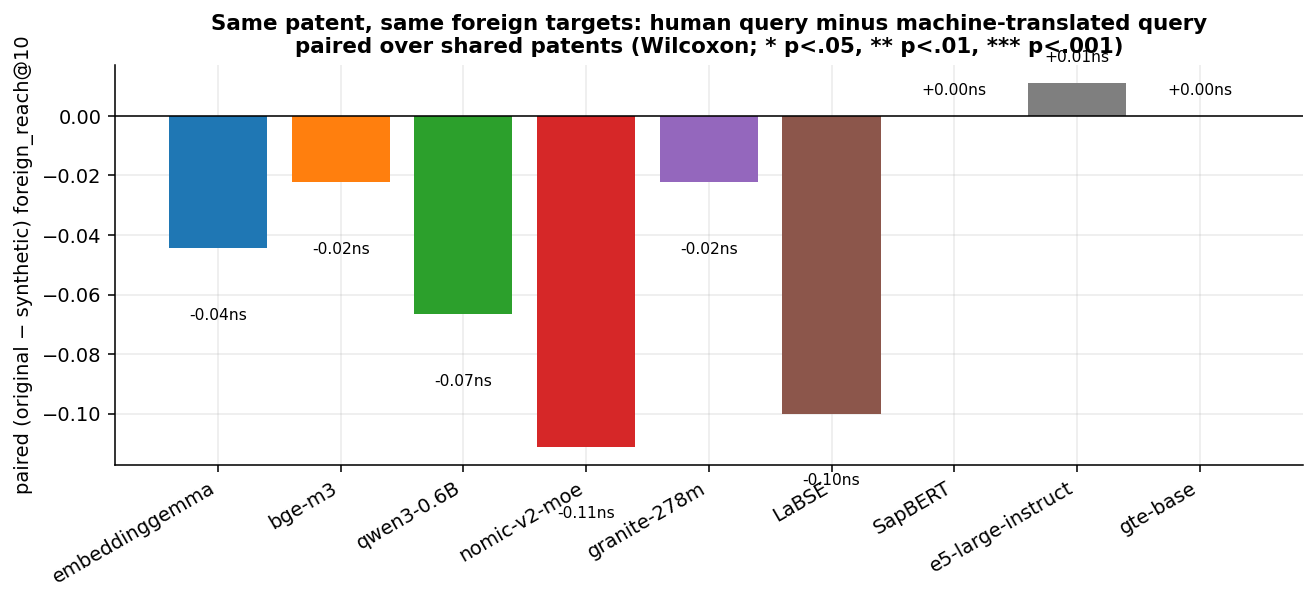
\includegraphics[width=\linewidth]{cp_fig05_mt_penalty.png}
  \caption{Human-written versus machine-translated queries. This supports the
  paper's practical separation between generating query variants and relying on
  human-translated source evidence.}
  \label{fig:app-mt-penalty}
\end{figure}

\begin{figure}[t]
  \centering
  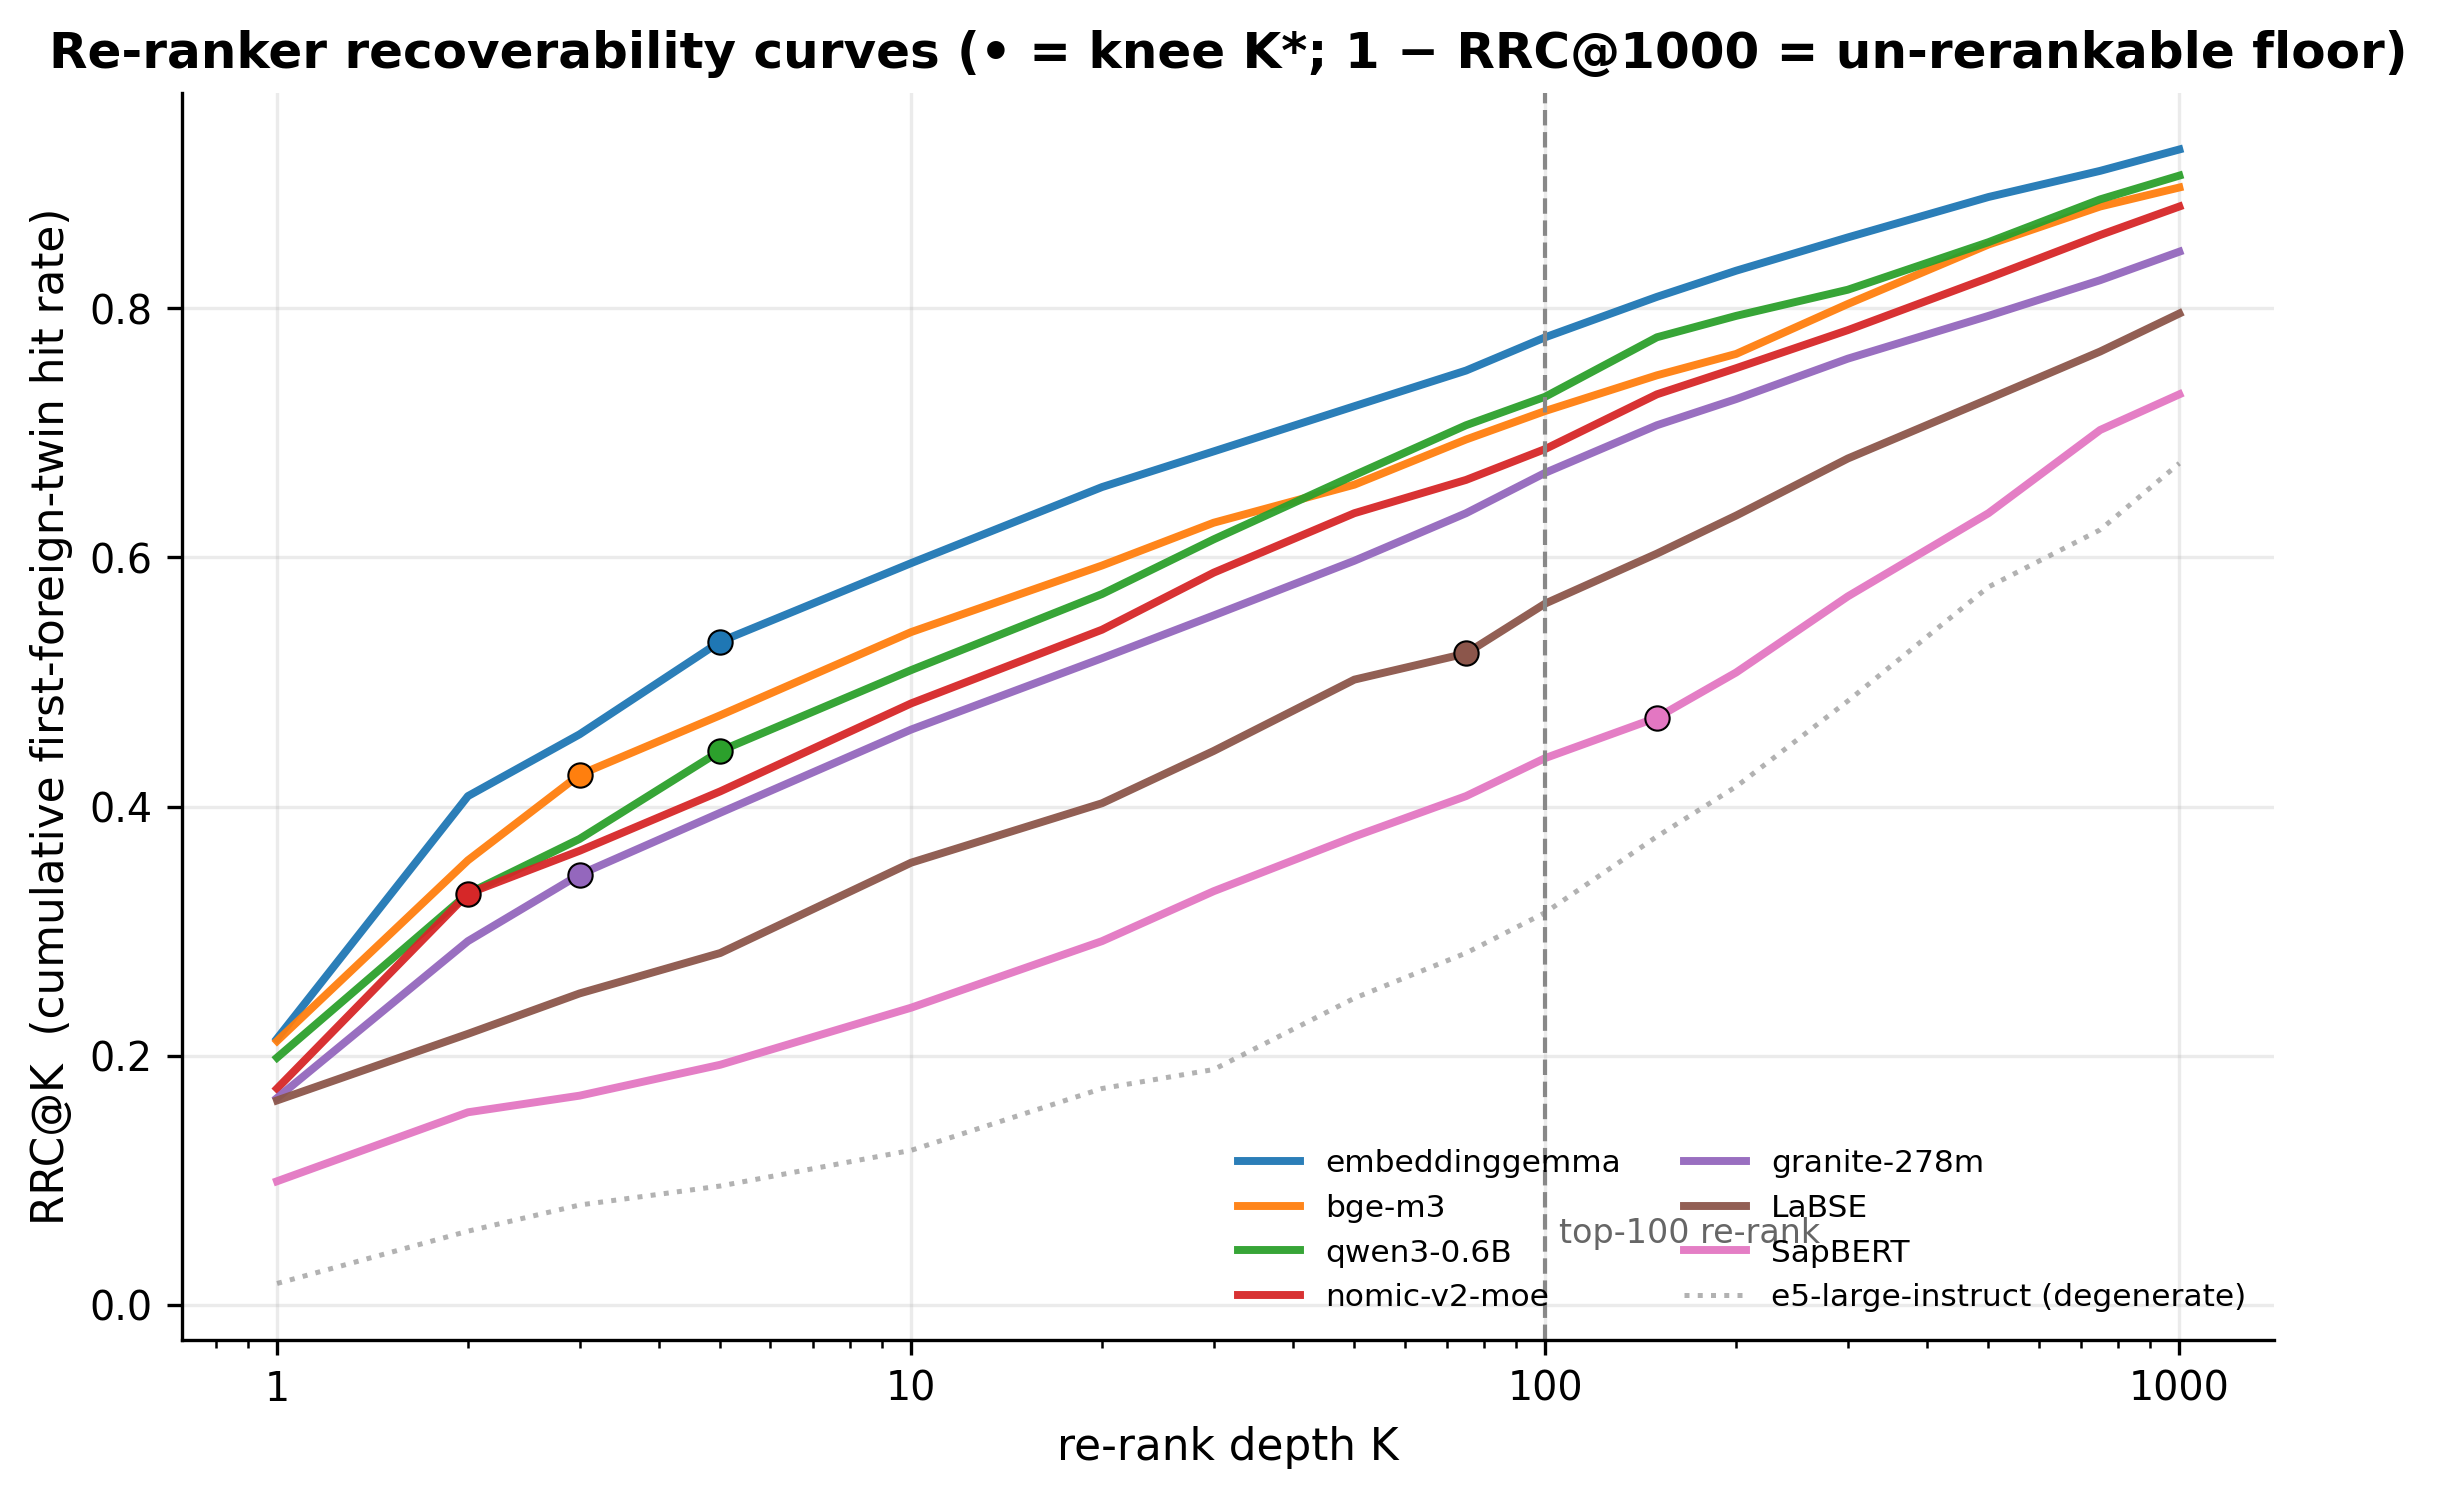
\includegraphics[width=\linewidth]{cp_fig19_rrc_budget.png}
  \caption{Re-ranker recoverability curves. These curves show how much
  cross-language evidence is recoverable at different candidate-pool depths and
  why some failures must be fixed before re-ranking.}
  \label{fig:app-rrc-budget}
\end{figure}


\end{document}
